
\documentclass [MS] {uclathes}
\usepackage{amsmath}
\usepackage{booktabs}
\usepackage{graphicx}
\usepackage{multirow}
\usepackage{url}
\usepackage{longtable}
\usepackage{caption}
\usepackage{subfig}

\graphicspath{ {./images/} }

\captionsetup{width=7in}

% \input {mymacros}                         % personal LaTeX macros

%%%%%%%%%%%%%%%%%%%%%%%%%%%%%%%%%%%%%%%%%%%%%%%%%%%%%%%%%%%%%%%%%%%%%%
%
% Usually things live in separate flies.
%
% \input {prelim}                           % preliminary page info

%%%%%%%%%%%%%%%%%%%%%%%%%%%%%%%%%%%%%%%%%%%%%%%%%%%%%%%%%%%%%%%%%%%%%%%%
%                                                                      %
%                          PRELIMINARY PAGES                           %
%                                                                      %
%%%%%%%%%%%%%%%%%%%%%%%%%%%%%%%%%%%%%%%%%%%%%%%%%%%%%%%%%%%%%%%%%%%%%%%%

\title          {Beating the Book: \\
                A Machine Learning Approach to NBA Win Probabilities \\
                in Search of an Edge Over the Betting Odds}
\author         {Guy Dotan}
\department     {Statistics}
% Note:  degreeyear should be optional, but as of  5-Feb-96
% it seems required or you get a year of ``2''.   -johnh
\degreeyear     {2020}

%%%%%%%%%%%%%%%%%%%%%%%%%%%%%%%%%%%%%%%%%%%%%%%%%%%%%%%%%%%%%%%%%%%%%%%%

\chair          {Frederic R. Paik Schoenberg}
\member         {Vivian Lew}
\member         {Zili Liu}

%%%%%%%%%%%%%%%%%%%%%%%%%%%%%%%%%%%%%%%%%%%%%%%%%%%%%%%%%%%%%%%%%%%%%%%%

%\dedication     {\textsl{To my mother \ldots \\
%                who---among so many other things--- \\
%                saw to it that I learned to touch-type \\
%                while I was still in elementary school}}

%%%%%%%%%%%%%%%%%%%%%%%%%%%%%%%%%%%%%%%%%%%%%%%%%%%%%%%%%%%%%%%%%%%%%%%%

\acknowledgments {(Acknowledgments omitted for brevity.)}

%%%%%%%%%%%%%%%%%%%%%%%%%%%%%%%%%%%%%%%%%%%%%%%%%%%%%%%%%%%%%%%%%%%%%%%%

%\vitaitem   {1974--1975}
%                {Campus computer center ``User Services'' programmer and
%                consultant, Stanford Center for Information Processing,
%                Stanford University, Stanford, California.}
%\vitaitem   {1974--1975}
%                {Programmer, Housing Office, Stanford University.
%                Designed a major software system for assigning
%                students to on-campus housing.
%                With some later improvements, it is still in use.}
%\vitaitem   {1975}
%                {B.S.~(Mathematics) and A.B.~(Music),
%                Stanford University.}
%\vitaitem   {1977}
%                {M.A.~(Music), UCLA, Los Angeles, California.}
%\vitaitem   {1977--1979}
%                {Teaching Assistant, Computer Science Department, UCLA.
%                Taught sections of Engineering 10 (beginning computer
%                programming course) under direction of Professor Leon
%                Levine.
%                During summer 1979, taught a beginning programming
%                course as part of the Freshman Summer Program.}
%\vitaitem   {1979}
%                {M.S.~(Computer Science), UCLA.}
%\vitaitem   {1979--1980}
%                {Teaching Assistant, Computer Science Department, UCLA.}
%\vitaitem   {1980--1981}
%                {Research Assistant, Computer Science Department, UCLA.}
%\vitaitem   {1981--present}
%                {Programmer/Analyst, Computer Science Department, UCLA.}

%%%%%%%%%%%%%%%%%%%%%%%%%%%%%%%%%%%%%%%%%%%%%%%%%%%%%%%%%%%%%%%%%%%%%%%%

%\publication    {\textsl{MADHOUS Reference Manual.}
%                Stanford University, Dean of Student Affairs
%                (Residential Education Division), 1978.
%                Technical documentation for the MADHOUS
%                software system used to assign students to
%                on-campus housing.}

%%%%%%%%%%%%%%%%%%%%%%%%%%%%%%%%%%%%%%%%%%%%%%%%%%%%%%%%%%%%%%%%%%%%%%%%

\abstract       {Lorem ipsum dolor sit amet, consectetur adipiscing elit. Nunc tincidunt dui eros, id tincidunt tellus mattis in. Morbi eget sem nec libero congue ultrices. Mauris dictum enim ut nisl iaculis, eu placerat leo sodales. Nam consectetur fringilla mi et facilisis. Cras egestas nisi eu scelerisque sollicitudin. Etiam sit amet nibh ligula. Aenean euismod tristique ante in eleifend. Mauris nibh nulla, consectetur ac mi ut, tempus suscipit leo. Maecenas vehicula consequat arcu eget feugiat. \\

Donec sed urna nec neque gravida elementum. Nullam turpis odio, venenatis sit amet feugiat dapibus, molestie eget quam. Phasellus justo enim, congue ut risus in, hendrerit posuere nibh. Quisque ultrices euismod pulvinar. Pellentesque eu facilisis libero. Phasellus efficitur porttitor ex vitae aliquam. Morbi metus ipsum, tempor quis lacus sed, interdum tincidunt mauris. Aliquam eget sollicitudin urna. Maecenas et ligula eget nibh maximus finibus. Maecenas justo turpis, rhoncus sit amet posuere at, pulvinar vitae purus. Nunc sed odio dui.}

%%%%%%%%%%%%%%%%%%%%%%%%%%%%%%%%%%%%%%%%%%%%%%%%%%%%%%%%%%%%%%%%%%%%%%%%


\begin {document}
\makeintropages

%%%%%%%%%%%%%%%%%%%%%%%%%%%%%%%%%%%%%%%%%%%%%%%%%%%%%%%%%%%%%%%%%%%%%%
%
% Ordinarily each chapter (at least) is in a separate file.
%
%\input {chapter1}                         % Chapter 1 of dissertation
%\input {chapter2}                         % Chapter 2
%\input {chapter3}                         % etc.
%\input {chapter4}
%\input {chapter5}
%\input {chapter6}
%\input {chapter7}
%\input {chapter8}

%      Chapter 1     %%%%%%%%%%%%%%%%%%%%%%%%%%%%%%%%%%%%%%%%%%%%%%%%%%%%%%%%%%%%
\chapter{Introduction}

The world of sports analytics has progressed rapidly over the past decade and with these advances, the entire professional sports landscape has evolved with it. While general advances in technology and sports organizations' willingness to pursue analytical research has facilitated the evolution, two seminal shifts within the field stand out as reasons for this surge. The first: the proliferation and democratization of accessible data. The second, and more recently: the federal legalization of sports gambling within the United States.

The sports industry is one of the newest sectors to be disrupted by the emergence of data-driven decision making challenging preconceived notions from ``experts'' and its impact has been fast and far reaching. Setting aside the unprecedented shock to the economic ecosystem---specifically within sports and entertainment---from the 2020 outbreak of COVID-19, the sports analytics business has been thriving. ``The global sports analytics market is expected to reach a revenue of \$4.5 billion by 2024, growing at a CAGR [Compound Annual Growth Rate] of 43.5\%.'' \cite{samf2024} 

\section{Current State of Sports Analytics}
To the general public, the most well-known adoption of analytics into the sports universe was within Major League Baseball, thanks largely to Michael Lewis' 2003 book \emph{Moneyball} and subsequent movie blockbuster, staring Brad Pitt, in 2011. The story chronicles the influence of Bill James, the field of empirical baseball research known as Sabermetrics, and the story of the 2002 Oakland A's unlikely success. \emph{Moneyball} has been the poster child of how data can create a competitive edge on the playing field. But sports analytics has made its impression in far more avenues than just baseball. The field is responsible for the increased emphasis of the three-point shot in basketball, the use of optical player tracking technology in the NFL, and even the statistical optimization of curling game strategy that helped the Swedish women's national team to a gold medal in the 2018 Winter Olympics \cite{curling}, just to name a few. 

The integration of data analysts and scientists as a crucial members of professional sports organizations appears here to stay, and the acceleration in the field's adoption can be tied to the increased availability of data. The NFL and NBA hold yearly hackathons to allow anyone the opportunity to dive into their sport's data and present findings to top league officials with prizes and networking at stake. Conferences such as the Sloan Sports Analytics Conference in Boston began as a small gathering of about 100 attendees in 2006, and now, in 2020, attracts over 4,000 people. The conference has gained national recognition, notably hosting former President Barack Obama as the keynote speaker in 2018. The industry's explosion in popularity though, has been aided by communities such as FiveThirtyEight, Retrosheet, Sports-Reference, and league-offered APIs bestowing data democracy to anyone that desires. Sports analytics has largely become open-source and this hive mind has benefited players, teams, and franchises. 

 \section{The Legalization of Sports Gambling}
On May 14, 2018, the Supreme Court case \emph{Murphy v. National Collegiate Athletic Association} reached a landmark decision regarding the federal government's right to control a state's ability to sponsor sports betting. In a 6-3 decision, the Professional and Amateur Sports Protection Act of 1992 (PASPA) was overturned, thus opening the doors for every state to make its own laws permitting in-state sports wagering. 

In just two years since the ruling there are already 18 states with full-scale legalization and another six that have passed legislation that will take effect in the coming year. \cite{betmap} And as one would expect, bettors in legal states have flocked to sportsbooks, both digital and brick-and-mortar. (Sportsbooks, or ``books'', are places, often times part of a greater casino, where bettors can make wagers on all types of sporting events.) Since the overturning of PASPA, Americans have placed over \$20 billion of bets which has generated \$1.4 billion of revenue in those legal states. \cite{betrevenue} Morgan Stanley projects that in just five years, by 2025, almost three-quarters of US states (36) will have legalized sports betting and the U.S. market could see \$7 to \$8 billion in revenue. \cite{market} 

\begin{figure}[h]
\centering
  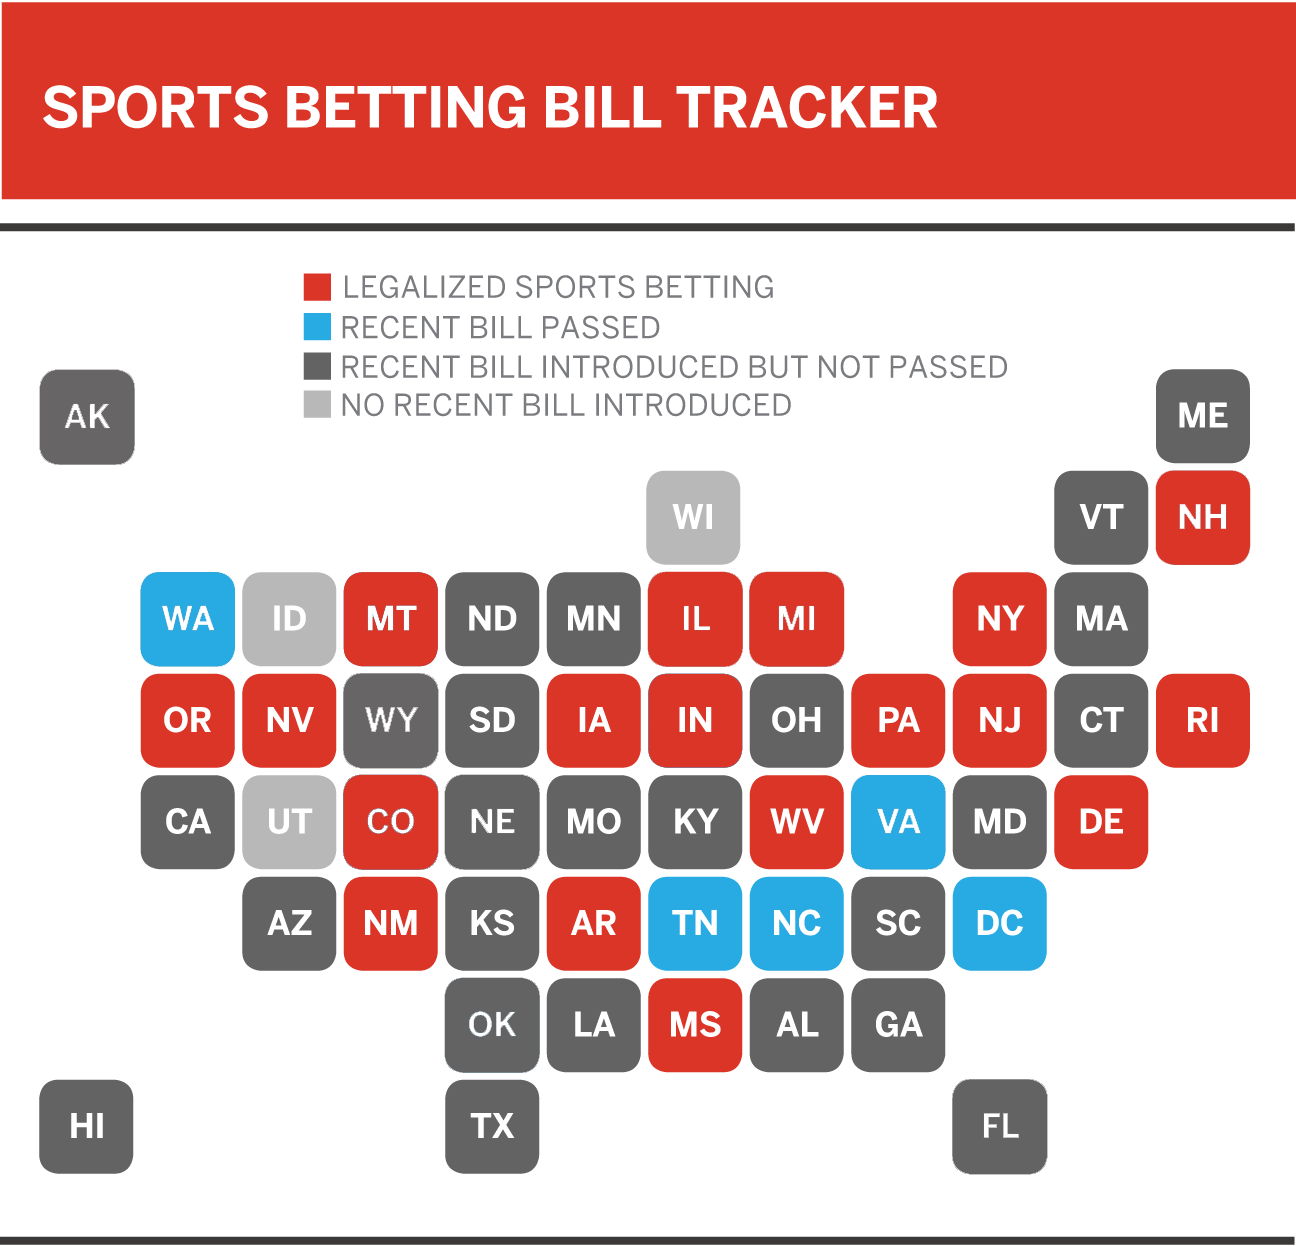
\includegraphics[width=250px]{20200520_betting_map.png}
  \caption{U.S. map of the current state of sports gambling legislation (as of May 2020)}
\end{figure}

\section{The Intersection of Data and Wagering}
Sportsbook operators within casinos have had decades of experience building a complex infrastructure of analytics to help them determine where to set their gambling lines. Their goal is to establish betting odds in a matchup such that there is an even amount of money wagered on both sides of the bet. This allows them to take their cut of the wagers (known in the industry as the ``vigorish'' or ``vig'') and thus drive revenue to their casino, no matter which team wins. For the entirety of their existence, sportsbooks have maintained a significant edge over the majority of bettors. Their advantage was largely based on their access to data and domain expertise building models to establish the perfect betting line. It is this statistical edge that has keeps income flowing into the sportsbooks within casinos. Money that helps build lavish 50-story casinos and hotels that make the Las Vegas strip world-renowned. That said, surprisingly, sports wagering makes just 3\% of gaming revenue in Nevada casinos. \cite{nevgame} 

\begin{figure}[h]
\centering
  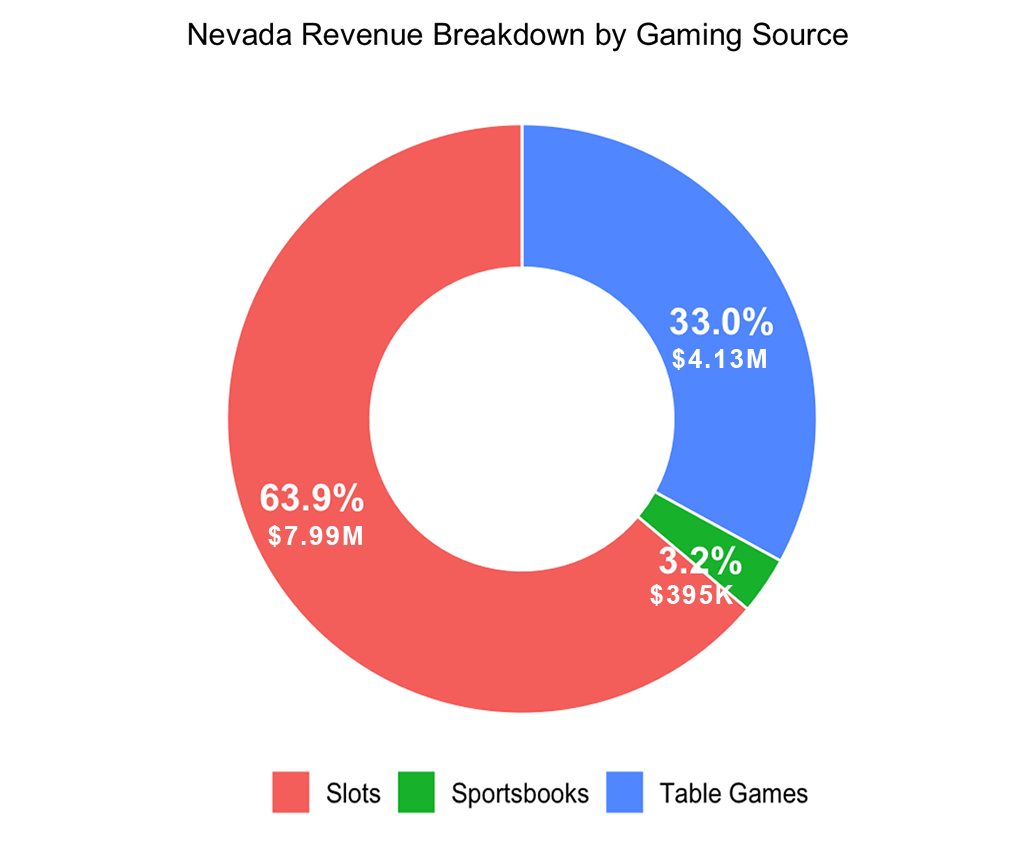
\includegraphics[width=300px]{gaming_revenue.png}
  \caption{Total gaming revenue by source in Nevada from Mar. 1, 2019 to Feb. 29, 2020}
\end{figure}

But now, with sports wagering becoming more commonplace in the American society and the proliferation of available sports data to everyday consumers, there is an opportunity to close the gap between casinos and bettors. Similar to how stockbrokers use proprietary projection models to systematically ``beat the market'', sports wagering has followed suit. 

Recall, a sportsbook's objective on each bet is to account for an even amount of money wagered on both sides. Often times a betting line is skewed by the inherent biases of an average sports bettor. For example, if the Los Angeles Lakers (a TV market size of over five million people) were to play the San Antonio Spurs (TV market size of just 900 thousand), we might expect a sportsbook to place the line so it slightly favors the Spurs. Even if the teams were evenly matched, sportsbooks would anticipate a disproportionate amount of hometown favorite bets supporting the Lakers. Just the smallest marginal edge, demonstrated by this example, could be enough to be exploited by an adept model. A model, when applied to a large enough dataset, could yield a considerate return on investment. 

The goal of this study is to determine if applying machine learning methods to vast sports datasets (in this case, within the NBA) can create such a model that would give a bettor the competitive edge over the lines set by a sportsbook. 


%      Chapter 2     %%%%%%%%%%%%%%%%%%%%%%%%%%%%%%%%%%%%%%%%%%%%%%%%%%%%%%%%%%%%
\chapter{The Mathematics of Sports Gambling}

In order to understand how to beat the bookmakers, one first needs to understand how to interpret the betting lines they provide. There is a wide array of different types of bets that a person can make at a sportsbook. The three most popular betting styles are: ``point spreads'', ``over/unders'', and ``moneylines''. This chapter will go into detail with descriptions of these types of bets using basketball as an example.

\section{Point Spreads, Over/Unders, and Moneylines}
Point spreads are mechanisms used to account for the discrepancy between two unevenly matched teams. Usually noted as: \emph{Warriors (-5) vs. Clippers} or the inverse: \emph{Clippers (+5) vs. Warriors.} The number in the parenthesis is called the ``spread.'' Essentially, the sportsbook believes that the Warriors are more likely to win the game, but the book wants to drive an even amount of bettors to wager on the Clippers (even though they are underdogs) as the Warriors. Therefore, the bookmakers suggest placing a spread of five points on the game. So, if you bet on the Warriors they need to win by more than 5 points to win the bet. If you bet on the Clippers, they have to lose by 4 points or fewer or win the game, for you to cash in on the wager. If the game ends with the Warriors winning by 5 points, then this is called a ``push'' and all bettors get their money back. Sometimes a spread will be listed at 0 points (called a ``pick-em''), indicating that this is an even matchup and all you have to do is pick the winner to win the bet.

Similar to point spreads, over/unders involve a specific point amount that a bettor needs to wager on the correct side of. However, in this case, the winner of the game is irrelevant. All the bettor must do is guess if the combined score between the teams will be greater than or less than the over/under line. For example, \emph{Warriors vs. Clippers (+200)}. If you bet the ``over 200'', you are expecting the combined score between the two teams to reach 201 or more and it does not matter what combination in occurs (Warriors 120-Clippers 81, Clippers 101-Warriors 100, etc.) If the final combined score is exactly 200, again this is called a push and bettors get their money back. For this reason, over/unders (and spreads for that matter), oftentimes use fractional lines (+5.5 or o200.5) to prevent the case of a push. Over/unders can be offered for single quarters, just the first half, just the second half, or even for a single team's score.

The third type of popular betting type are called moneylines and are the subject of this study. In a moneyline bet, a person simply needs to determine which team will win the game. But if one team was the heavy favorite versus the other team, it would not make sense for a sportsbook to pay out an equal amount for choosing the favorite as choosing the underdog. As a result, sportsbooks offer a moneyline, which adjusts the amount you win for having your bet hit based on the likelihood that team will win the game. Moneylines are notated in various formats: decimal, fractional, and moneyline. The first two are commonly used in Europe. This paper will use the moneyline odds notation since they are most common to the US (and often called ``American'' odds). Moneylines are written as follows: \emph{Warriors (-235) vs. Clippers}, or conversely, \emph{Clippers (+185) vs. Warriors.} 

Essentially, these either positive or negative, three-digit numbers, imply how much money a bettor would profit relative to a \$100 bet. +185 means that if a bettor laid \$100 on the Clippers, and then they won the game, the bettor would make \$185 profit. -235 means that a bettor would have to wager \$235 in order to profit \$100 from that game. So if a bettor placed \$100 on the Warriors at -235 moneyline odds, and the Warriors indeed won, the bettor makes \$42.55 profit. 

\noindent \text{\underline{Moneyline Profit - Underdog}} \\
\text{Let $Profit_{dog} = \Pi_{d}$ } \\
\begin{equation} \label{ml_prof_dog}
\begin{split}
\frac{ML}{100}  & = \frac{\Pi_{d}}{Risk}  \\
100*\Pi_{d} & = ML*Risk    \\
\Pi_{d} & = \frac{ML}{100} * Risk 
\end{split}
\end{equation}

\noindent \text{Using our example...}
\begin{equation*} 
\begin{split}
\Pi_{d} & = \frac{+185}{100} * 100 \\
 & = 1.85 * 100 \\
 & = \$185
\end{split}
\end{equation*}


\noindent \text{\underline{Moneyline Profit - Favorite}} \\
\text{Let $Profit_{fav} = \Pi_{f}$ } \\
\begin{equation} \label{ml_prof_fav}
\begin{split}
\frac{-1 * ML}{100}  & = \frac{Risk}{\Pi_{f}}  \\
\Pi_{f} * (-1 * ML) & = Risk * 100  \\
\Pi_{f} & = \frac{100}{(-1 * ML)} * Risk 
\end{split}
\end{equation}

\noindent \text{Using our example...}
\begin{equation*} 
\begin{split}
\Pi_{f} & =  \frac{100}{(-1 * -235)} * 100 \\
 & = \frac{100}{235} * 100 \\
 & = .4255 * 100 \\
 & = \$42.55
\end{split}
\end{equation*}

In summary, a \$100 bet on the Clippers (+185) leads to \$185 profit. A \$100 bet on the Warriors (-235) leads to about \$42 profit. This discrepancy in profits is to discourage enough bettors from taking the favorite Warriors and instead take the potential for upside in profit by betting on the underdog Clippers. Again, the sportsbooks goal is to optimize these moneylines to set it at a line such that an even amount of money is placed on both sides. 

\section{Implied Win Probability}
The payout formula for moneylines makes it quite simple to determine how much profit a bettor can make from having their wager hit. Risk averse bettors tend to take favorites (negative moneylines) despite the lower payouts because there is a higher chance that the team they bet on will win. Risky bettors will seek out underdogs (positive moneylines) with lower probabilities of winning, but they think will actually surprise the public, win the game, and thus provide a larger profit-margin. 

In addition to the payout, however, moneylines can actually be converted into a win probability known as ``implied probability''. The implied probability formula is defined as the size of the bettor's wager divided by the return on investment for that wager. Or simply: risk over return. When placing a wager and consequently winning that wager, the bettor receives their initial risk amount back in addition to the profit-margin. Thus, return on investment of a wager is just risk plus return.

\begin{equation} \label{imp_prob}
\begin{split}
& Implied Probability = \frac{Risk}{Return}  \\
\end{split}
\end{equation}
Note: \emph{Return} = \emph{Risk} + \emph{Profit}

\section{Derivation of Implied Win Probability}
A universal formula to calculate the implied win probability for any bet (underdog or favorite) can be derived by plugging in the formula for moneyline profit for an underdog (equation \ref{ml_prof_dog}) and a favorite (equation \ref{ml_prof_fav}) into the implied probability formula (equation \ref{imp_prob}).

\noindent \text{\underline{Implied Probability - Underdog}} \\
\begin{equation} \label{ip_dog}
\begin{split}
IP_{dog} & = \frac{Risk}{Return}  \\
& = \frac{Risk}{Risk + \Pi_{d}}  \\
& = \frac{Risk}{Risk + \left( \frac{ML}{100}*Risk \right)} \\ 
& = \frac{Risk}{Risk \left( 1 + \frac{ML}{100}  \right)} \\ 
& = \frac{1}{ 1 + \frac{ML}{100} } \\ 
IP_{dog} & = \frac{100}{100 + ML} 
\end{split}
\end{equation}


\noindent \text{\underline{Implied Probability - Favorite}} \\
\begin{equation} \label{ip_fav}
\begin{split}
IP_{fav} & = \frac{Risk}{Return}  \\
& = \frac{Risk}{Risk + \Pi_{f}}  \\
& = \frac{Risk}{Risk + \left( \frac{100}{-1 * ML} * Risk \right) } \\ 
& = \frac{Risk}{Risk \left( 1 + \frac{100}{-1 * ML}  \right)} \\ 
& = \frac{1}{ 1 + \frac{100}{(-1 * ML)} } \\ 
IP_{fav} & = \frac{(-1 * ML)}{(-1 * ML) + 100} 
\end{split}
\end{equation}

\noindent \text{\underline{Implied Probability - General Equation}} \\
\begin{equation} \label{ip_gen}
\text{IP(ML) =}
\begin{cases}
\displaystyle
 \frac{100}
 {ML * 100},  & \text{if ML} \geq 0 \\ \\ 
\displaystyle
 \frac{(-1 * ML)}
 {(-1 * ML) +100}, &  \text{if ML} <  0\\ 
\end{cases}
\end{equation}

\section{The Vig or the Juice}
As mentioned previously, the goal of a sportsbook is to have an equal amount of money placed on both sides of a wager so that no matter the results, they will make money once they take their cut of the bets. This cut is known as the vigorish, and more colloquially, the ``vig'' or the ``juice.'' So how does one calculate the juice? Let's use our example from above with the Warriors versus the Clippers.

The Warriors moneyline odds were -235, which after using Formula \ref{ip_gen}, comes out to an implied probability of 70.15\%. The Clippers moneyline odds were +185 and therefore an implied probability of 35.09\%. Now, the most basic rule of probability states that the sum of all possible outcomes of an event always equals 1. And more specifically, the probability of an event plus the probability of the complement of that event equals 1. In basketball there are only two valid outcomes of a game: win or loss. If we consider the chances that a team wins a game as the probability while the chances they lose is the complement of that probability, we would expect these two events to sum to 1. See below: \\ 

\noindent \text{\underline{Given:}} \\
\noindent \text{$P(A) + P(A^{c}) = 1 $ } \\
\noindent \text{Let ...} \\
\noindent \text{$P(A)$ =  Probability that Warriors win } \\
\noindent \text{$P(A^{c})$ = Probability that Warriors lose (i.e. Clippers win)} \\
\noindent \text{$P(A)$ =  0.70 } \\
\noindent \text{$P(A^{c})$ =  0.35 }
\begin{flalign*}
P(A) + P(A^{c}) & =  &&\\
0.70 + 0.35 & = 1.05 &&\\ 
1.05 & \neq 1
\end{flalign*}

So these two implied probabilities are mutually exclusive, compose the entire space of outcomes, and yet sum to over 100\%. This summed probability (in this case 105\%) that is greater than 1 is called the ``overround'' and is how sportsbooks take their cut. By setting the betting lines such that the probabilities result in an overround, the sportsbook effectively ensures that they will gain a profit from this wager. In our example above, a \$100 bet on the Warriors pays out \$42, while a \$100 bet on the Clippers pays out \$185. One can determine how much a sportsbook would expect to pay out from these implied probabilities through the following calculation:

\noindent \text{\underline{Expected Profit:}} \\
\noindent \text{Let $E(\Pi) $ = Expected Profit for Sportsbook} \\
\noindent \text{$E(\Pi_i) = \Pi_i * P(win_i) $ } \\
\noindent \text{ $E(\Pi) = \sum_i{\Big( E(\Pi_{i}) \Big) } $} \\
\noindent \text{ $E(\Pi) = \sum_i{\Big( \Pi_i * P(win_i) \Big) } $} \\
\noindent \text{ $E(\Pi) = \Pi_A * P(win_A) + \Pi_{A^C} * P(win_{A^C}) $} \\

\noindent \text{Using our example...} \\
\noindent \text{$E(\Pi_A) $ = Expected Profit if Warriors Win} \\
\noindent \text{$E(\Pi_{A})  = \Pi_{A} * P(A)$} \\
\noindent \text{$E(\Pi_A) $ = $\sim $\$42 * 0.7 = $\sim$\$30} \\
\noindent \text{$E(\Pi_{A^C}) $ = Expected Profit if Clippers Win} \\
\noindent \text{$E(\Pi_{A^C})  = \Pi_{A^C} * P(A^C)$} \\
\noindent \text{$E(\Pi_{A^C}) $ = \$185 * 0.35 = $\sim$\$65} \\
\noindent \text{$E(\Pi)$ = \$30 + \$65 } \\
\noindent \text{= $\sim$\$95} \\


As seen above, this overround (105\%) of the probabilities creates the vig for the casino. If the sportsbook were to take \$100 of total wagers on this bet, on average, they would expect to pay out just \$95. Thus, ensuring a cut of about \$5 for this wager. Now consider the fact that casinos collect millions of dollars on bets, not \$100, it is easy to see why sports gambling is such a lucrative endeavor for bookkeepers, especially when the optimal moneylines are established (and therefore the juice is optimized as well). \\

\section{``Removing the Juice'' - Actual Win Probability}
In order to get a clear idea of the sportsbooks' expectations of how likely each of the two teams is to win a matchup, we need to get rid of the guaranteed profit they bake into the lines. The implied probabilities are derived from the betting lines, but the actual probabilities are what remains after taking the vig into account. Probability theory claims that the sum of all possible events in a sample space should always equate to 1. So to get the true probabilities based on the betting odds, the implied probabilities need to be scaled so that they also sum to 1. The method to remove the vig is simple, just divide the probability by the overround. \cite{vig}\\

$$
\displaystyle
Actual Probability = \frac{Implied Probability}
{Overround}
$$

$$
\text{Actual Probability the Warriors Win} = \frac{70\%}{105\%} = 67\% \\
$$
$$
\text{Actual Probability the Clippers Win} = \frac{35\%}{105\%} = 33\% \\
$$

We see that the two probabilities now sum up to 100\% and therefore represent the true probability that the sportsbook places on each team's chances of winning. In summary: \\

\begin{table}[ht!]
\caption{Summary of betting values for sample wager}
\label{tab:bet-summary-table}
\resizebox{\textwidth}{!}{%
\begin{tabular}{@{}lrrrrrr@{}}
\toprule
Team     & \multicolumn{1}{l}{Moneyline Odds} & \multicolumn{1}{l}{Risk} & \multicolumn{1}{l}{Profit} & \multicolumn{1}{l}{Return} & \multicolumn{1}{l}{Implied Win Probability} & \multicolumn{1}{l}{Actual Win Probability} \\ \midrule
Warriors & -235                               & \$100                    & \$42                       & \$142                      & 70\%                                        & 67\%                                       \\
Clippers & +185                               & \$100                    & \$185                      & \$285                      & 35\%                                        & 33\%                                       \\ \bottomrule
\end{tabular}%
}
\end{table}


%      Chapter 3     %%%%%%%%%%%%%%%%%%%%%%%%%%%%%%%%%%%%%%%%%%%%%%%%%%%%%%%%%%%%
\chapter{Data Collection}

The gambling mathematics discussed in Chapter 2 can be applied to any sport with betting lines. But for this study, we focused specifically on professional basketball betting data. The NBA is a particularly useful test subject for this research for a few reasons. First off, over the last decade, the NBA has experienced arguably the largest increase in the emphasis put on data analytics of the four major sports (NHL --- hockey, MLB --- baseball, and NFL --- football). More interest in basketball analytics has led to easier accessibility to data that could be useful for research and modeling.

Not only is the data availability trending upwards, but the general popularity of the sport of basketball is on the rise as well. A 2017 Gallup poll found that basketball has surpassed baseball as America's second-most favorite sport to watch. Although, football is still heavily the favorite: at 37\%, versus 11\% for basketball. \cite{gallup} Thus, with the sport's popularity continuing upwards one would expect the betting markets to grow as well. 

\begin{figure}[h]
\centering
  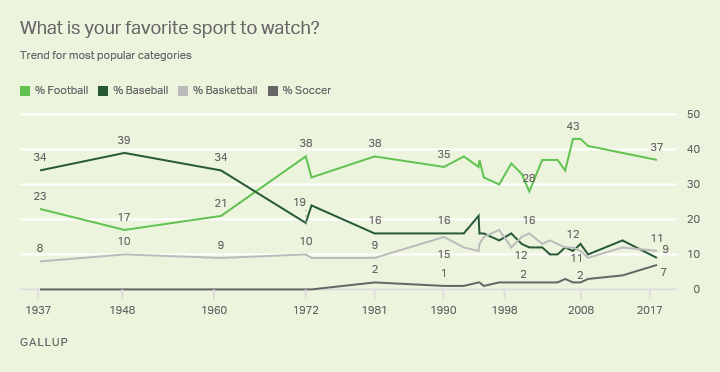
\includegraphics[width=350px]{fav_sports.png}
  \caption{Survey from Gallup on Americans and their favorite sport to watch}
\end{figure}

Additionally, for our purposes, the advantage the NBA has over the NFL, is its sample size. The NBA consists of 30 teams and an 82-game season, as opposed to the NFL which has 32 teams, but teams play just 16 games in the regular season. Additionally, basketball games are high scoring and high possession competitions, hence, within a single basketball game, there are a lot of statistics that accumulate. Much more than a baseball, football, or hockey game. Simply put: lots of games and lots of stats within those games makes for a large sample size and a great dataset.

\section{Betting Lines}
The first step to building the dataset required for this study was acquiring betting data for as many NBA games as possible. More specifically, we are looking for moneylines odds since that is what is necessary to convert betting lines into win probabilities. Fortunately, an archive of betting odds for the NFL, NBA, NCAA football, NCAA basketball, MLB, and NHL were all available on one online resource.\footnote{https://sportsbookreviewsonline.com/scoresoddsarchives/scoresoddsarchives.htm} The relevant data for this study went back to the 2007-08 NBA season and was complete up to the current 2019-20 season. Each file was formatted into one of 13 downloadable Excel files that contained both regular and postseason odds. Each season's data was clean and uniform, which seamlessly merged into one large dataset of 32,952 rows (16,476 games since each game had two rows to represent each team's odds). There were no missing moneylines in the dataset, spanning from the first game of the 2007-08 season until the NBA season was abruptly cut short on March 11, 2020. This was a historic day, not only in basketball, but professional sports history. Before tipoff, Rudy Gobert, a center for the Utah Jazz tested positive for COVID-19, prompting commissioner Adam Silver to cancel Utah's game versus the Oklahoma City Thunder and then the rest of the season indefinitely. \cite{nbacovid} 

With a complete set of betting data, the final processing step for the dataset was to convert those odds into win probabilities. Using the derived probability formulas from Chapter 2, R functions were written to implement these formulas and were systematically applied to the entire betting dataset. 

\section{NBA Game Statistics}
There were several different approaches for statistics that we could use to build a win probability model to pair alongside our archive of betting odds. The most straightforward approach, and the one used for this research, was to utilize game-by-game, team-level box scores. Game-level detail allowed for the flexibility to aggregate the data in a variety of ways that would be useful for modeling purposes.

Fortunately, the R package \emph{nbastatR} provides a robust interface that easily pulls data from an array of online basketball data resources such as: NBA.com/Stats, Basketball Insiders, Basketball-Reference, HoopsHype, and RealGM. \cite{nbastatr} One of the functions in this package loads game-logs for each team over any desired seasons. All that was necessary was to input the same 2007-2020 season span that we already had in our betting archive. This gave us the same 16 thousand or so games and over two dozen raw team statistical variables to use in our model. A data dictionary of these variables is shown in Table \ref{tab:nba-vars}. 

Joining the betting odds data with the game-log box scores was not a trivial task. Because these datasets did not come from the same source there was no linking key between each box score, each betting line, and each team. However, through rigorous data cleaning---which included the manual creation of standardized team IDs and game IDs---we were able to combine the two datasets together. The merging of the two datasets was a perfect match with team statistics available for every single matchup in which betting lines were available, save two instances. One, the cancelled 2020 games due to COVID-19 and two, a March 15, 2013 game between the Boston Celtics and Indiana Pacers which was cancelled, and never rescheduled, as a result of the tragic bombing at the Boston Marathon the day before. \cite{si} 

\footnotesize
\begin{longtable}{@{}lll@{}}
\caption{Data dictionary of variables from betting archive and NBA box scores}
\label{tab:nba-vars}\\
\toprule
Category & Variable & Description \\* \midrule
\endfirsthead
%
\endhead
%
\bottomrule
\endfoot
%
\endlastfoot
%
\multirow[t]{10}{*}{Matchup} & \texttt{idGame} & (num) Unique game ID \\
 & \texttt{slugSeason} & (num) NBA season \\
 & \texttt{gameDate} & (date) Date of the game \\
 & \texttt{beforeASB} & (T/F) Game is before All-Star Break (T) or after (F) \\
 & \texttt{locationGame} & (char) Home or away \\
 & \texttt{slugMatchup} & (char) Game matchup \\
 & \texttt{slugTeam} & (char) Team abbreviation \\
 & \texttt{slugOpponent} & (char) Opponent team abbreviation \\
 & \texttt{numberGameTeamSeason} & (num) Team's Xth game of season \\
 & \texttt{isB2B} & (T/F) Is the team on a back-to-back (i.e. 0 days rest) \\
 & \texttt{isB2BFirst} & (T/F) First game of a back-to-back \\
 & \texttt{isB2BSecond} & (T/F) Second game of a back-to-back \\
 & \texttt{countDaysRestTeam} & (num) Number of days since the team's last game \\
 & \texttt{countDaysNextGameTeam} & (num) Number of days until the team's next game \\* \midrule
\multirow[t]{4}{*}{Outcome} & \texttt{slugTeamWinner} & (char) Winning team abbreviation \\
 & \texttt{slugTeamLoser} & (char) Losing team abbreviation \\
 & \texttt{outcomeGame} & (char) Team win or loss \\
 & \texttt{isWin} & (T/F) Team win or loss \\* \midrule
\multirow[t]{4}{*}{Betting Odds} & \texttt{teamML} & (num) Moneyline odds for the team \\
 & \texttt{oppML} & (num) Moneyline odds for the opponent \\
 & \texttt{teamWinProb} & (num) Win probability for the team \\
 & \texttt{oppWinProb} & (num) Win probability for the opponent \\* \midrule
\multirow[t]{23}{*}{Traditional Stats} & \texttt{fgmTeam} & (num) Field goals made by the team \\
 & \texttt{fgaTeam} & (num) Field goals attempted by the team \\
 & \texttt{pctFGTeam} & (num) Field goal percentage from team \\
 & \texttt{fg3mTeam} & (num) 3PT field goals made by the team \\
 & \texttt{fg3aTeam} & (num) 3PT field goals attempted by the team \\
 & \texttt{pctFG3Team} & (num) 3PT field goal percentage by the team \\
 & \texttt{pctFTTeam} & (num) Free throw percentage by the team \\
 & \texttt{fg2mTeam} & (num) 2PT field goals made by the team \\
 & \texttt{fg2aTeam} & (num) 2PT field goals attempted by the team \\
 & \texttt{pctFG2Team} & (num) 2PT field goal percentage by the team \\
 & \texttt{minutesTeam} & (num) Minutes played by the team \\
 & \texttt{ftmTeam} & (num) Free throws made by the team \\
 & \texttt{ftaTeam} & (num) Free throws attempted by the team \\
 & \texttt{orebTeam} & (num) Offensive rebounds by the team \\
 & \texttt{drebTeam} & (num) Defensive rebounds by the team \\
 & \texttt{trebTeam} & (num) Total rebounds by the team \\
 & \texttt{astTeam} & (num) Total assists by the team \\
 & \texttt{stlTeam} & (num) Total steals by the team \\
 & \texttt{blkTeam} & (num) Total blocks by the team \\
 & \texttt{tovTeam} & (num) Total turnovers by the team \\
 & \texttt{pfTeam} & (num) Personal fouls committed by the team \\
 & \texttt{ptsTeam} & (num) Total points scored by the team \\
 & \texttt{plusminusTeam} & (num) Differential in the team score (Own - Opponent points) \\* \midrule
\multirow[t]{2}{*}{Advanced Stats} & \texttt{possessions} & (num) True team possessions in a game \\
 & \texttt{pace} & (num) Number of possessions per 48 minutes by a team. \\* \bottomrule
 \end{longtable}

\normalsize

\section{Advanced Metrics}
For the majority of basketball history, analytics were driven by these standard box score metrics currently in our dataset. More recently, however, the industry has been shifting away from these raw values toward a more dynamic approach that can take into account the shifts in game tempo season-to-season and even game-to-game. The solution: looking at the normal metrics---points, rebounds, assists, etc.---on a per possession basis, as opposed to per game. ``By looking at the game at a per-possession level, it eliminated pace and style of play differences from the equation and put all teams on a level playing field. This way a team that is constantly running and has more possessions each game doesn't have a statistical advantage compared to a team that plays at a slower speed.'' \cite{nbaadvstats} 

Possessions used to be estimated through a rudimentary formula that took into account how many field goals, free throws, turnovers, and rebounds a team got over the course of a game. But with the proliferation of play-by-play data, the NBA now has an exhaustive account for true possessions for each team and each game dating back to the 1996-97 season. The NBA actually provides advanced data (of which possessions is included) on a per game and per team basis through an open API.\footnote{Application Programming Interface}  Using Python's \emph{requests} package, we were able to tap into the API and then make the call to the appropriate endpoints to return a data dump of advanced metrics for each game. The data came in a JSON format, so all that was left to do was to use Python's \emph{pandas} library to format the JSON response into a data frame so it is easier to work with. Since this data was pulled directly from the NBA's official statistics database, the game IDs and team IDs directly matched those that came from the traditional box score metrics from the \emph{nbastatR} package and the two were successfully joined together. 

Our dataset was now complete with betting data (and corresponding win probabilities), matchup data (outcome, home/away, days rest, etc.), traditional box score metrics, and per-game possessions. 


%      Chapter 4     %%%%%%%%%%%%%%%%%%%%%%%%%%%%%%%%%%%%%%%%%%%%%%%%%%%%%%%%%%%%
\chapter{Data Processing and Exploratory Analysis}

The raw box score statistics provided the backbone for the features that will need to be included in the win probability model. With those box scores, we then applied two types of transformations to our dataset. The first, as mentioned previously, was to scale the raw metrics to account for the variability in game-to-game possessions. The second, was to aggregate the data to account for the accumulation of statistics each team had built up entering the given matchup. 

\section{Seasonal Trends}

People who have been fans of the NBA over the past couple decades can attest to how different the game is played in 2020 than before. Whether it is due to the rise in analytics, improvements in training and medical advances, or gameplay strategy implemented by coaches, the fact remains: what it takes to win a basketball game has changed. One of the biggest shifts in game style recently has been the tendency to shoot more three pointers. The secret to unlocking this strategy is no real mystery. NBA teams on average shoot about 35\% on three pointers, 45\% on two pointers, and 75\% on free throws. The math breaks down quite simply as follows: 

\noindent \text{\underline{Expected Points on a Certain Shot Attempt:}} \\
\noindent \text{Expected Points = (Points) * (Percent changes of making the shot)} \\
\noindent \emph{E(3PA)} = 3 * 0.35 = 1.05 \\
\noindent \emph{E(2PA)} = 2 * 0.45 = 0.90 \\
\noindent \emph{E(FTA)} = 1 * 0.75 = 0.75

There are obviously more subtleties and complexities to these style changes, but the redefining of the ideal shot selection distribution has been a major component. With these types of optimizations occurring on the court, we see it manifesting in season-wide trends on the box score metrics. Figure \ref{fig:statstrends} demonstrates these trends. 

\begin{figure}[h]
\centering
  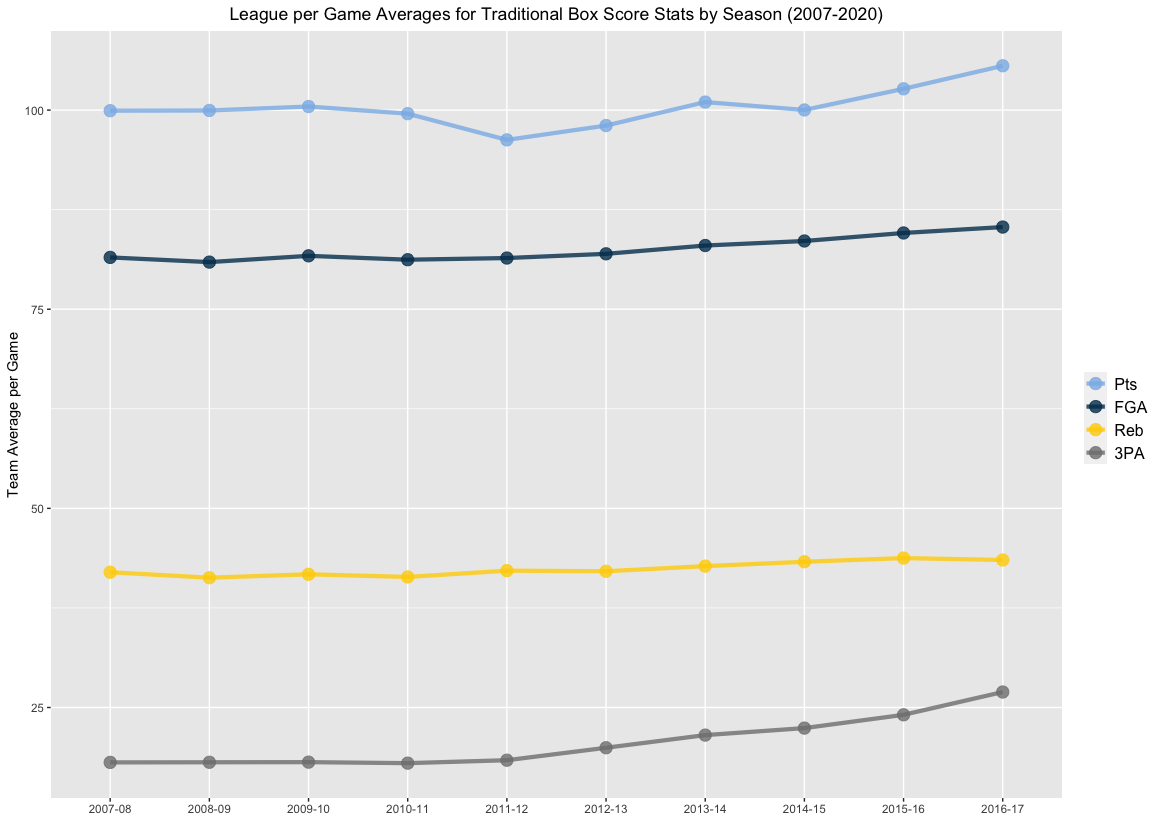
\includegraphics[width=500px]{stats_season_avg.png}
  \caption{Statistical trends by season}
  \label{fig:statstrends}
\end{figure}


All four of these metrics are trending upwards, with the most drastic increase being three-point attempts. Just to accentuate this point, the team with the fewest three-point attempts per game in 2019-20 (the Indiana Pacers at 27.5 per game), would have ranked first place by almost a full three-point attempt per game in the 2007-08 season (the Golden State Warriors ranked first with 26.6 per game). The NBA-leading Houston Rockets, who averaged 44.3 threes per game in 2019-20, calculate out to a 145\% increase in three-point attempts compared to the league average 18.1 attempts in 2007-08. Going further, 48\% of the Rockets field-goal attempts this year came from behind the arc, compared to the league average of 22\% back in 2007-08. The league average in 2019-20 was 38\%. 

Three pointers are up, shooting attempts are up, scoring is up, rebounding is up, all of today's traditional box score metrics are inflated compared to earlier in the decade. The question that emerges is whether this inflation is due to optimizations in offensive schemes or merely a change in the flow of the game. The eye test suggests that the NBA game is much faster paced today than it was a decade ago. As it turns out, the data backs this belief up. 

The more possessions a team gets in a game, the higher tempo that game is being played at. The basketball statistic ``pace'' is defined as the average of both team's possessions per 48 minutes of combined game play. \\

\noindent $$ \text{Pace = }  48 * \frac{(TmPoss + OppPoss)}{2 * (TmMin / 5)}  $$ 

The season-to-season trend in pace verifies our assumption that the game is played at a higher velocity today. Figure \ref{fig:pace} shows the positive slope on the regression of pace by season demonstrated as both a scatterplot and series of box plots. \\

\begin{figure}[h]
\centering
  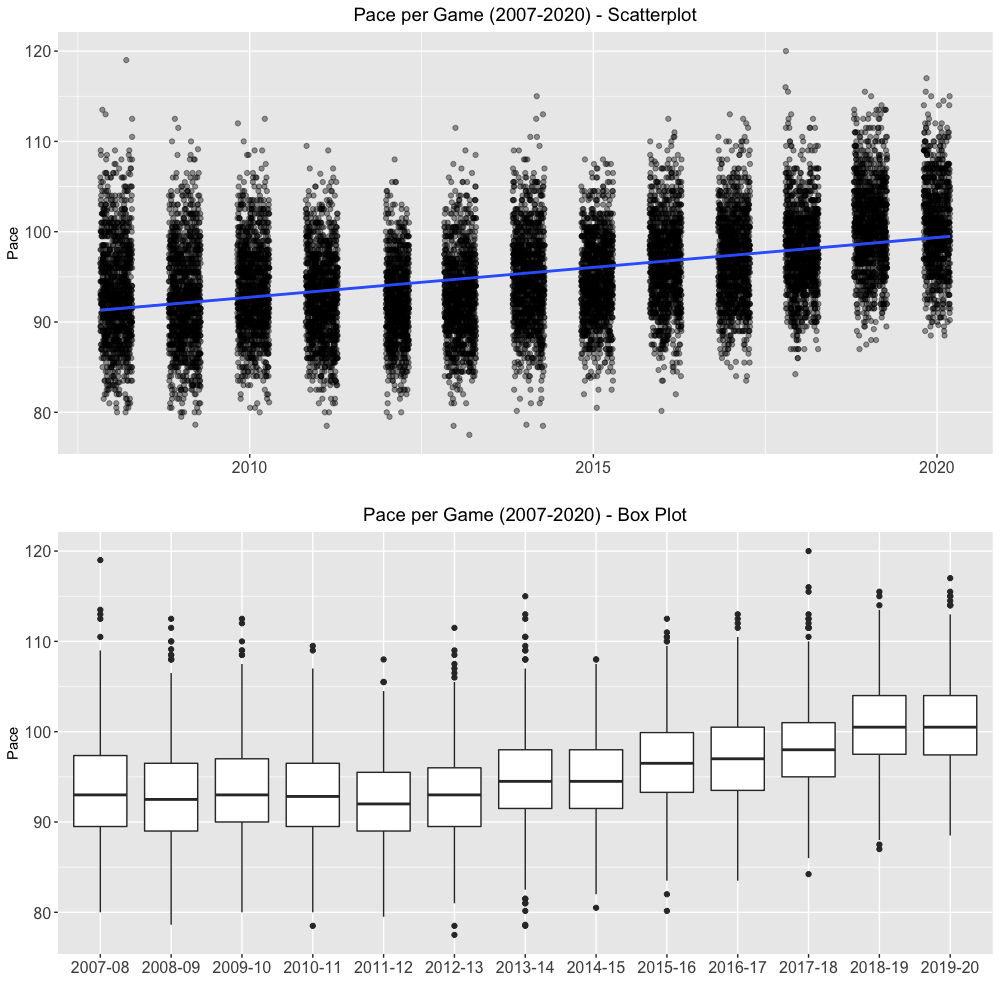
\includegraphics[width=400px]{pace_byseason.png}
  \caption{Team pace by season}
  \label{fig:pace}
\end{figure}


\section{Adjusting for Pace}

The solution that the basketball analytics community has put in place to combat this phenomenon of statistical inflation is pace-adjusted metrics. Instead of aggregating stats on a per-game basis, we now examine those same stats in relation to how many possessions that team had in the game. More specifically, the standardized pace-adjusted metric looks at a team's stats per 100 possessions. Previously, adjusting statistics on a per-48-minute basis was used to account for overtime games, but using per-100 possessions addresses both overtime instances as well as seasonal and daily shifts in game play. 

When we build our model, it is important to handle this inflation factor as we don't want a ``good'' team back in 2007 to appear like a ``bad'' team by 2020 standards. The top two charts in Figure \ref{fig:paceadjust} show the distribution of scoring and field goal attempts for all games in the 2007-08 season versus the 2019-20 season. As is apparent, the 2019-20 season is shifted to the right verifying this statistical inflation. However, when scaling these two metrics onto a per-100 possessions scale, we see a far greater overlap between the two distributions. Clearly, the increase in pace does not account for the entirety of the scoring surges, but it does lessen the gap. 

\begin{figure}[h]
\centering
  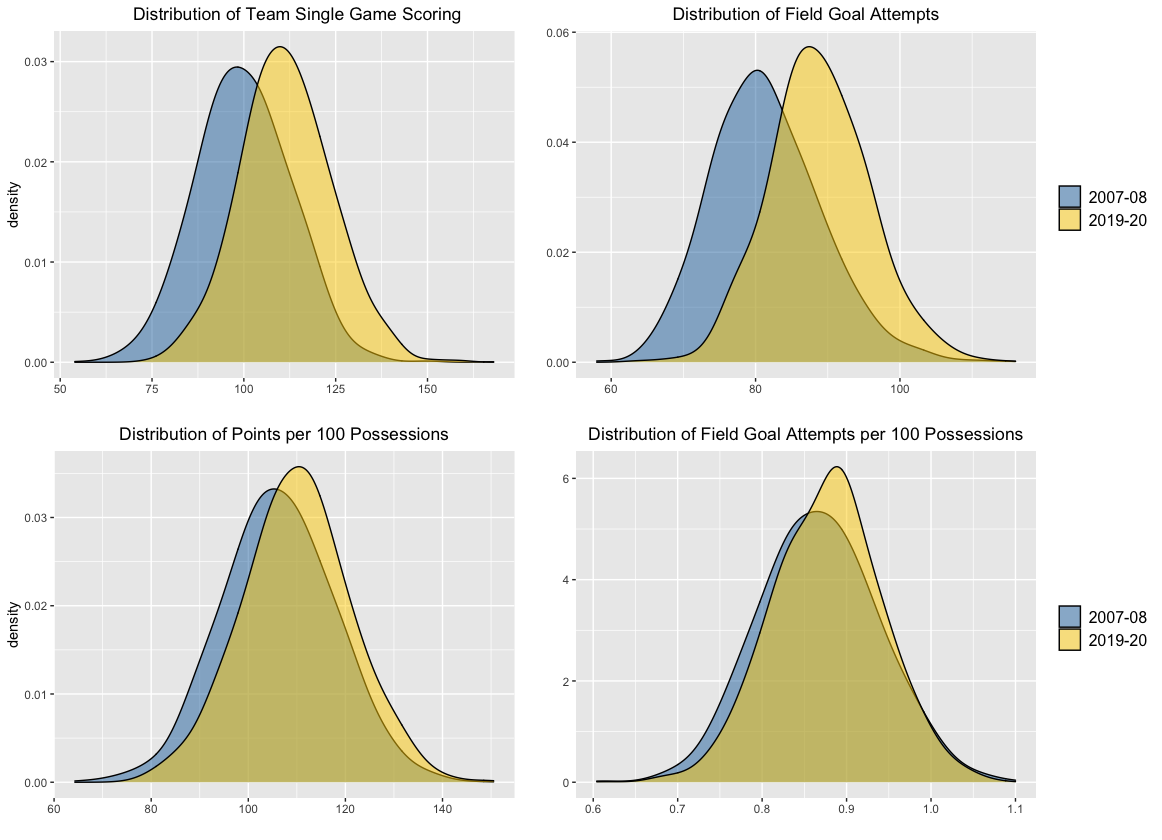
\includegraphics[width=500px]{pace_adjust_hist.png}
  \caption{Pace adjusted metrics, 2007-08 vs. 2019-20}
  \label{fig:paceadjust}
\end{figure}

For the purposes of this research we will scale all of the standard box score metrics on a per-100 possession basis. This methodology will help dramatically when trying to train a dataset that spans over a long time frame by creating a standardization across the ever-changing styles of play. In fact, points scored per 100 possessions (Offensive Rating), points allowed per 100 possessions (Defensive Rating), and the difference between the two (Net Rating) are some of the key metrics used by the analytics community to define the quality of a team's performance. We revisit these ratings in the modeling sections later in this study. Figures \ref{fig:ortg}, \ref{fig:drtg}, \ref{fig:nrtg} paint a rather clear picture as to the correlation between the best teams in the league and their performance in those three advanced ratings. 

\begin{figure}[p]
\centering
  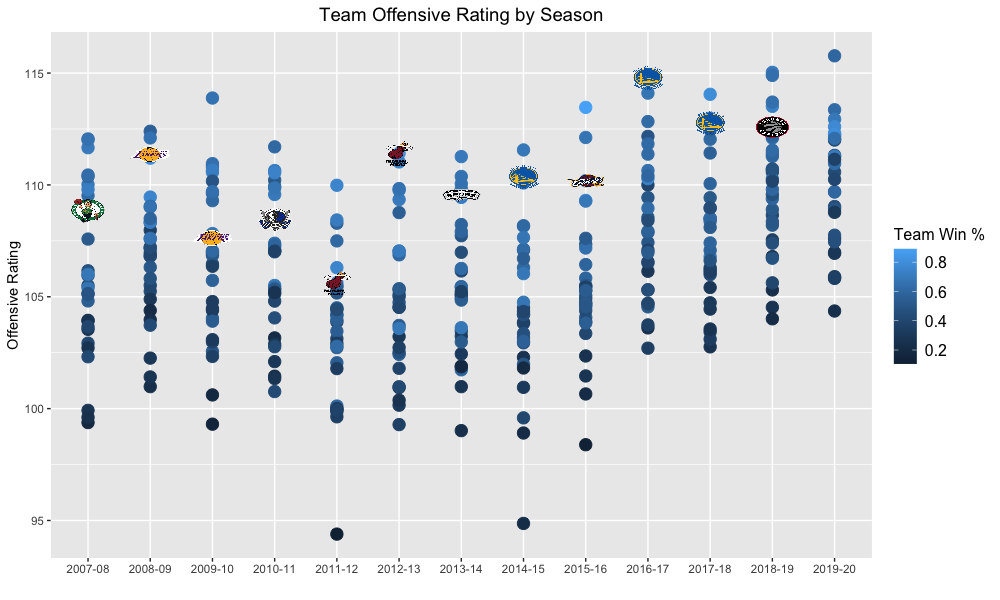
\includegraphics[width=450px]{off_rtg.png}
  \caption{Offensive rating by season (NBA champion indicated by team logo)}
  \label{fig:ortg}
  
\vspace{1cm}
  
\centering
  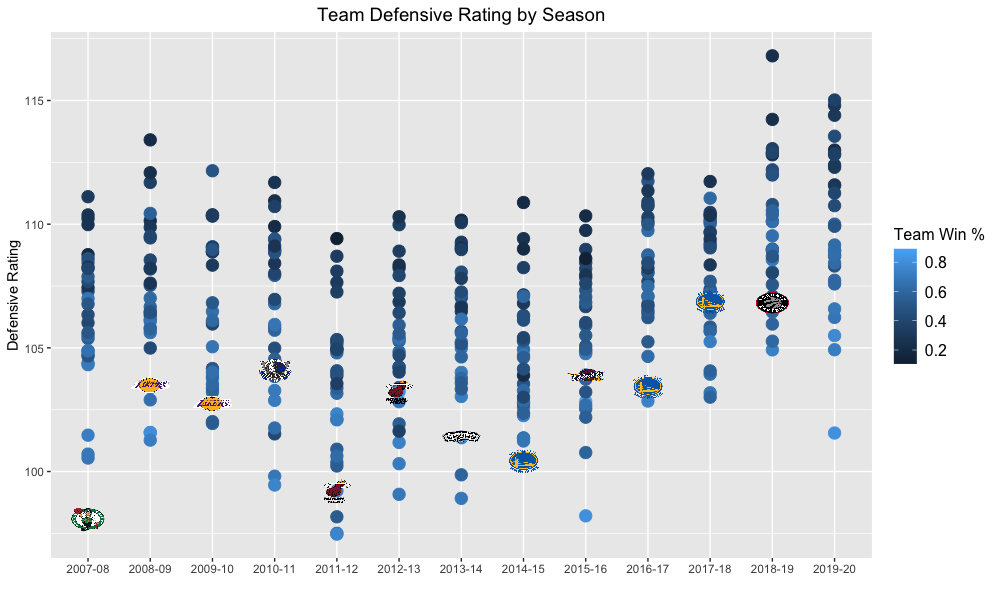
\includegraphics[width=450px]{def_rtg.png}
  \caption{Defensive rating by season (NBA champion indicated by team logo)}
  \label{fig:drtg}
\end{figure}

\begin{figure}[h]
\centering
  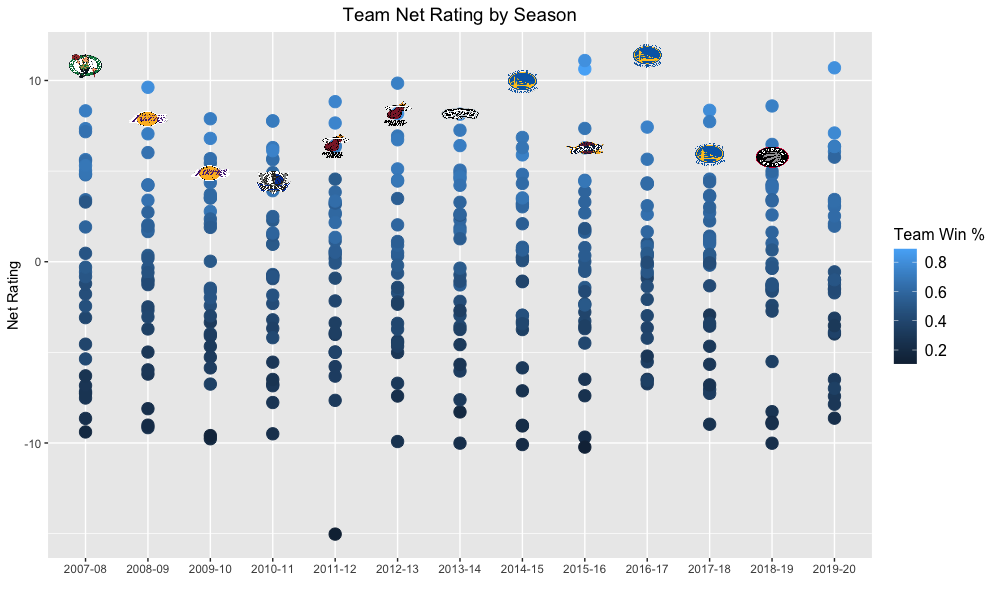
\includegraphics[width=450px]{net_rtg.png}
  \caption{Net rating by season (NBA champion indicated by team logo)}
  \label{fig:nrtg}
\end{figure}


\section{Aggregation}

A complete dataset of box scores and matchup details provides the opportunity for a lot of flexibility in how to best aggregate the data. Before aggregating though, there was more pre-processing required to handle all aspects for a team and their matchup. First off, the data had to be joined to itself so that we knew not only the team's own box score in that game, but also their opponent's. Access to the opponent's statistics for each matchup makes it much easier to understand the team's performance on both offense and defense. The number of points and offensive rebounds a team gets will be valuable in a model, but equally as valuable are the number of points they give up and offensive rebounds they allow. Also recall that opponent possessions were part of the formula for pace. 

Of course, the statistics that we need to consider when building the model to predict which team won, are not the team's performance in that game, but the games leading up to it. We took two different aggregation methods to our dataset. The first was the team's year-to-date performance entering that game. So, for example, if both teams were on their tenth game of the season, we had the first nine games worth of data aggregated for each squad to make a prediction on that matchup. If it was the last game of the season for both teams, we had 81 games worth of data for each. The one caveat: if the game was the first of the season for that team, we used the entire previous season's worth of data as our predictors.  

The second aggregation method took into account the ebbs and flows of a basketball season. Some teams go on hot streaks or cold streaks so using the entire season's stats to date might not be the best method. As an alternate aggregation option, we looked at the team's performance in the five-game span entering that game. This rolling aggregation would hopefully be more sensitive than the year-to-date method in reflecting how the team has been performing entering the matchup. The one caveat for this method: if it was the team's fifth game of the season or earlier, the aggregation would roll back to the previous season. So, if it was the team's third game of the year, the aggregation would consist of the first two games of that season and then the three last games of the previous. Again, all of these metrics in both methodologies were scaled on a per-100 possession basis, not as the combined raw totals within the aggregation period. 

The final processing step before building the model was required because of the unique response variable for this study. Our goal was to predict the probability that a team would win a game against its opponent, given all the data provided for that matchup. In order to properly build this model, we cannot treat both teams in that matchup as separate entities. If we did, there would be no way to guarantee that the combined win probabilities for both teams would sum to 100\%. Therefore, the proper way to transform our dataset would be to join the data to itself once again. By randomly assigning a ``1'' or ``2'' to each team in a matchup, we could merge \emph{Team 1's} data to \emph{Team 2's}, such that there is only one row per game. This randomization technique was a better strategy than dividing the dataset into home and away teams because we preserve the \texttt{locationGame} variable. History suggests the home team wins about 59\% of the time versus the away team and therefore location might be a useful predictor in our dataset. Consequently, this processing step allows us to structure the model so that the response variable (p) is the probability that the randomly defined \emph{Team 1} wins. Then we can simply find the probability that \emph{Team 2} wins by doing 1 - p. 

Thus, our dataset went from about 32,000 rows (one row per each team in the matchup) down to about 16,000 rows (one row per game). The sample size may have halved, but the parameter set quadrupled. Before we had just the team's own statistics for each game. After the processing we now had, for each aggregation technique:

\begin{enumerate}
\item Team 1's own statistics entering each matchup
\item Team 1's opponent's statistics entering each matc22hup
\item Team 2's own statistics entering each matchup
\item Team 2's opponent's statistics entering each matchup
\end{enumerate}

The last alteration to the dataset was to remove postseason games from this particular research. In the NBA postseason, teams play a best-of-seven-game series against the same team. In addition, the competition is much higher since only the eight best teams from each conference qualify. Therefore, top caliber teams would be losing more frequently than they normally would when playing the full spectrum of competition. Predicting the winner of postseason games is a critical aspect to a robust betting model, but in order to narrow the scope of this study, we will stick to regular season only. With that last step, these two datasets---the five-game rolling aggregates and the year-to-date statistics---were in a form ready for modeling. While the target response variable, to reiterate, was the binary classification of whether the randomly assigned \emph{Team 1} of the matchup won the game. 


%      Chapter 5     %%%%%%%%%%%%%%%%%%%%%%%%%%%%%%%%%%%%%%%%%%%%%%%%%%%%%%%%%%%%
\chapter{Model Building}

Before training any preliminary models, it was worthwhile to see if there was any redundancy in our variable set. A quick way to examine that potential is to look at correlations/multicollinearity within the numerical predictors in the dataset. Figure \ref{fig:corrs} shows the breakdown for all correlations between the single-team box score metrics in the modeling set, including the advanced ones. As one familiar with basketball statistics might expect, there were some quite highly correlated variables.

For example, we calculated pace earlier in the study as basically a per-48 minute transformation for possessions. And as a result, the correlation between he two variables was 0.9. Field-goal attempts was highly correlated with field-goals mades (0.8), free-throw attempts was associated to free-throws made (0.9), and total rebounds was correlated to defensive rounds (0.8). Additionally, all of the shooting percentage metrics (field-goal percentage, two-point field-goal percentage, etc.), were highly associated with the shooting attempts metrics. 

Clearly, many of the standard NBA box score statistics are interrelated, which is why the analytics communities have crafted advanced metrics that bake in many of these raws statistics into a catch-call measure. Examples of these are ``true shooting percentage'' and ``defensive rebounding percentage''.\footnote{https://www.basketball-reference.com/about/glossary.html} For further research, it would be prudent, to examine these advanced metrics developed by basketball's analytics community when building probability such as the one in this study. Regardless, for the purposes of this study, we will stick to our available box score metrics and keep in mind the opportunity to eliminate these correlated variables when choosing the best predictors for the model. 

\begin{figure}[h]
\centering
  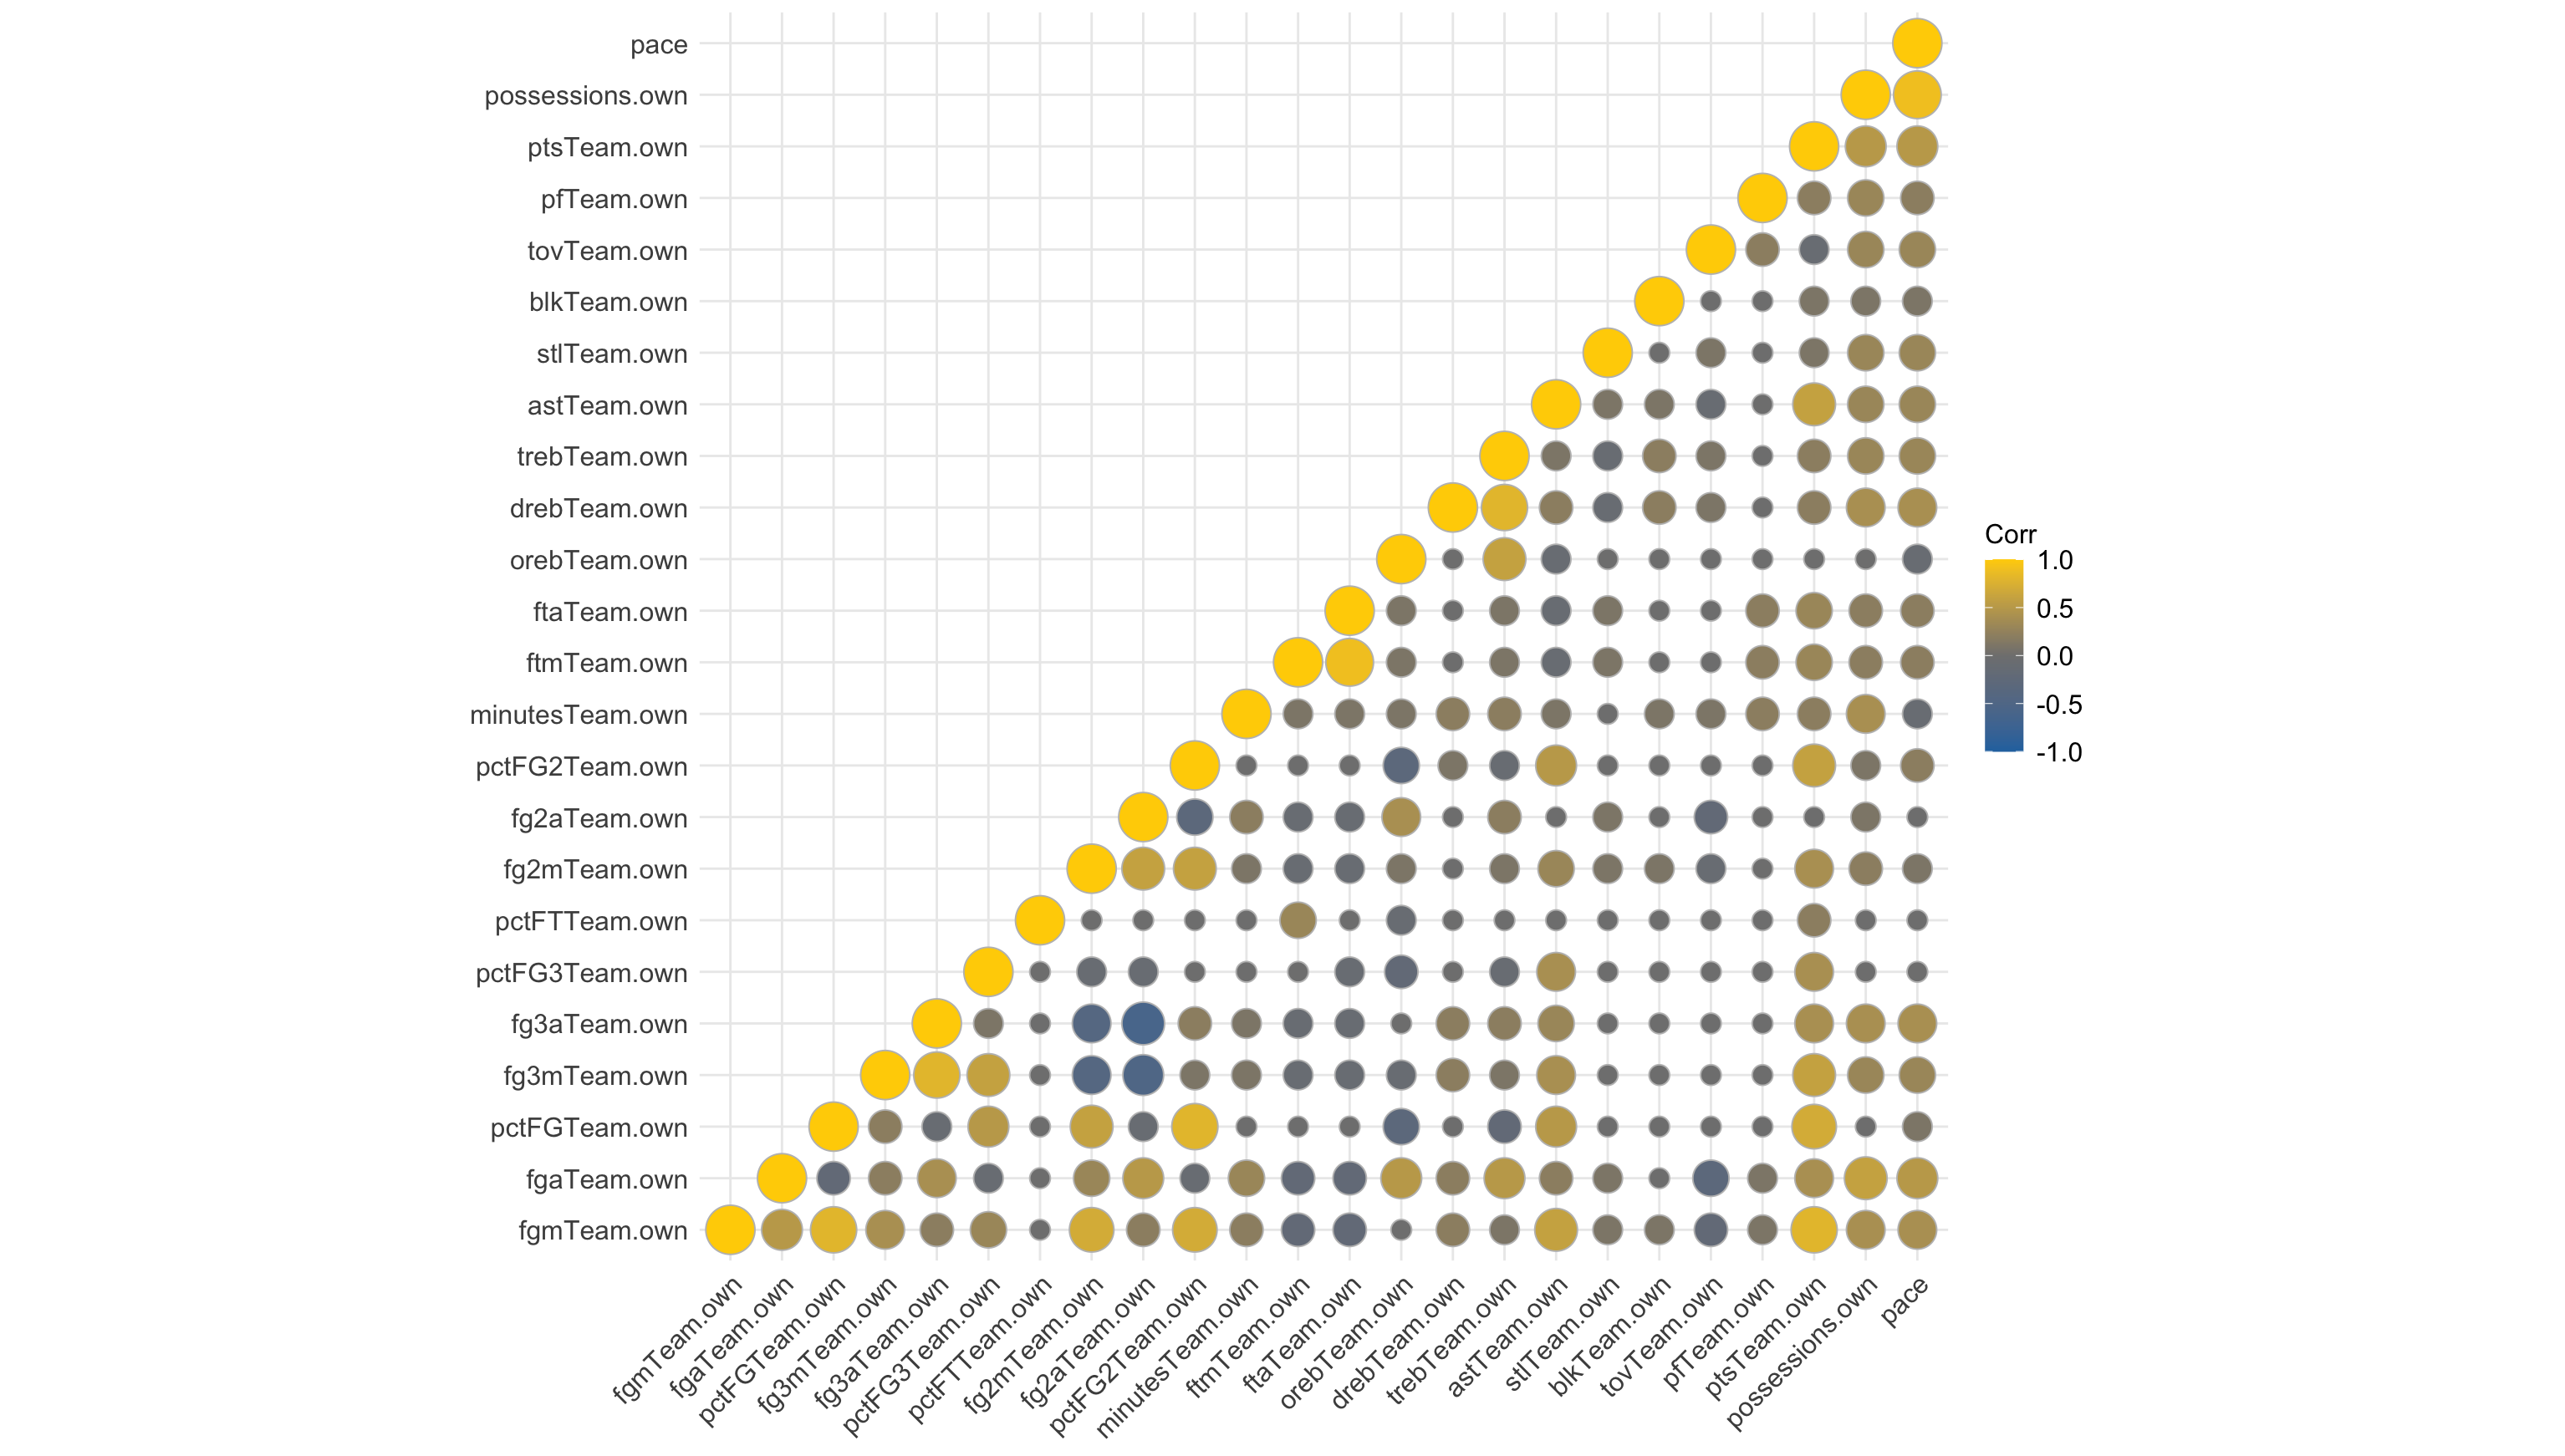
\includegraphics[width=500px]{corrs_plot.png}
  \caption{Correlation Matrix for Box Score Statistics}
  \label{fig:corrs}
\end{figure}


\section{Logistic Regression}
Since our response outcome is a binary variable (team 1 either won or lost) we would be remiss to not begin the model building process with an attempt at a logistic regression. The more common, linear regression, is ideal for scenarios where you are predicting an outcome that has a range of possibilities, usually continuous. How much revenue a product will sell or how long a flight might take, for example. Whereas with a logistic regression the predicted Y values are restricted by an asymptote that exists at 0 and at 1. Logistic regression is reserved for models with two outcomes, whether a patient tests positive or negative for a disease or will a person default on their credit or not.

In fact, for our particular study, logistic regression is a perfect model type to explore as it does not actually give you a single binary response. Logit models returns a probability score that reflects the predicted probability of the occurrence of that event. That probability is then rounded (usually at 50\%) to determine whether the model predicts a positive or negative response. Figure \ref{fig:logit} depicts a logistic regression curve and the range of outcomes that can be outputted from a model. 
 
\begin{figure}[h]
\centering
  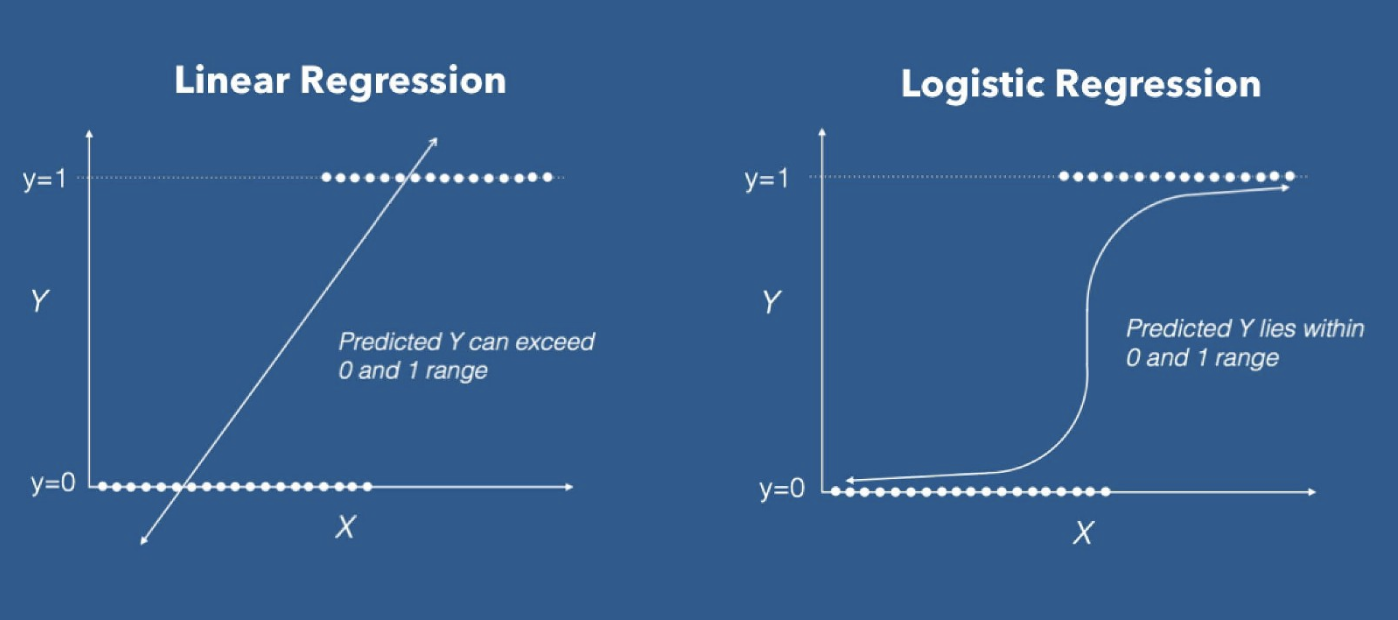
\includegraphics[width=400px]{logistic-reg.png}
  \caption{Simplified examples of a linear regression versus logistic regression}
  \label{fig:logit}
\end{figure}

Logistic models, and most machine learning algorithms, operate best when only the most critical features are included in the model. Reasons for this reality of model building are many, some of which being that fewer features allow for algorithms to train faster, improves interpretability of the final result, reduces overfitting, and when properly fewer features can actually improve the accuracy of model versus one with far more.

To conduct all of the model building in this study we used the \emph{caret} package with R. \emph{Caret} is short for ``classification and regression training'' and contains a variety of tools to prep the data for modeling, build training and testing sets, and has over 200 different machine learning algorithms available. But before diving into any the logistic models, the first step was to identify any potentially high importance features. Using \emph{Caret}, we implemented the recursive feature elimination technique to identify these best predictors.



\section{Random Forest}

\section{xGBoost}


%      Chapter 6     %%%%%%%%%%%%%%%%%%%%%%%%%%%%%%%%%%%%%%%%%%%%%%%%%%%%%%%%%%%%
\chapter{Neural Network}

%      Chapter 7     %%%%%%%%%%%%%%%%%%%%%%%%%%%%%%%%%%%%%%%%%%%%%%%%%%%%%%%%%%%%
\chapter{Beating the Book}

Recall, the intention of this research was not merely to perform a series of modeling experiments, determine the the most performant one, and then stop there. Our model evaluation process concluded the XXXX model performed best on the training and testing sets, but the true worth of this prognostication tool would be in its application to the real world: the betting markets. We had two hypotheses related to building a win probability model for NBA games. One, that the availability of data could allow anyone with the toolset to create a prediction system that could emulate what the sportsbook experts do on a daily basis in establishing their betting lines. Two, that inherent biases might exist within these lines based on factors outside of pure win expectancy that could lead to edges that could be exploited by an objective model.

Now, we do not need our model to perform significantly better than the professional sportsbook line setters, nor do we need there to be a considerable edge from irrational bettors to capitalize on. The magic number in sports betting is not 100\% as it is to perfectionists. Nor is it 99.7\%, 95\%, or 68\% as it is to the ``empirically-ruled'' Gaussians. In sports wagering, statistical significance for bettors actually lies at the all-important benchmark of 52.4\%. \cite{medium524}

\section{Why 52.4\% Matters}
Back in Chapter 2, we broke down the mathematics and economics of sports betting. We derived the formula to convert odds to both expected profit as well as win probabilities. From Equation \ref{ip_gen}, we can determine the moneyline that one would expect in a matchup between two evenly matched teams; that is, each team's chances of winning is 50\%. \\

\noindent \underline{Expected Moneyline for an Even Matchup:}
\begin{flalign*}
IP_{dog}(ML) &= \frac{100}{ML + 100} & \\
0.50 &= \frac{100}{ML + 100} \\
0.50 &= \frac{100}{ML + 100}  \\
0.50 * (ML +100) &= 100  \\
\frac{ML}{2} + 50 &= 100  \\
\frac{ML}{2} &= 50  \\
ML &= +100
\end{flalign*}

The same result occurs (-100 moneyline) if we set \emph{I(P)} equal to 0.50 in the formula for implied probability of a favorite. And these results make sense. If you were betting \$100 on a 50/50 coin flip, you would expect to get \$100 profit if your side landed face up. But of course, as referenced previously, sportsbooks always take their share of the betting pool---their vig. Typically,  for an even odds game, a sportsbook will take a 10\% cut of the betting margin. This means that you'd have to put in \$110 on a team in order to win \$100 (essentially a -110 moneyline). So in order to find the break-even point on a -110 moneyline payout we simply plot the return on investment percentage as your win probability increases, as shown in Figure \ref{fig:exp-val}.  \\

\noindent \underline{Return on Investment vs. Win Probability:}
\begin{flalign*}
& ROI = \frac{Expected Value}{Risk}  &
\end{flalign*}
\noindent \emph{EV} = \emph{P(W)} * \emph{Profit} - \emph{P(L)} * \emph{Risk}  \\
\noindent \emph{EV} = \emph{P(W)} * \$100 - \emph{P(L)} * \$110  \\
\noindent \emph{EV} = \emph{P(W)} * \$100 - (1 - \emph{P(W)}) * \$110 


\begin{figure}
  \begin{minipage}[c]{0.75\linewidth}
    \vspace{0pt}
    \centering
     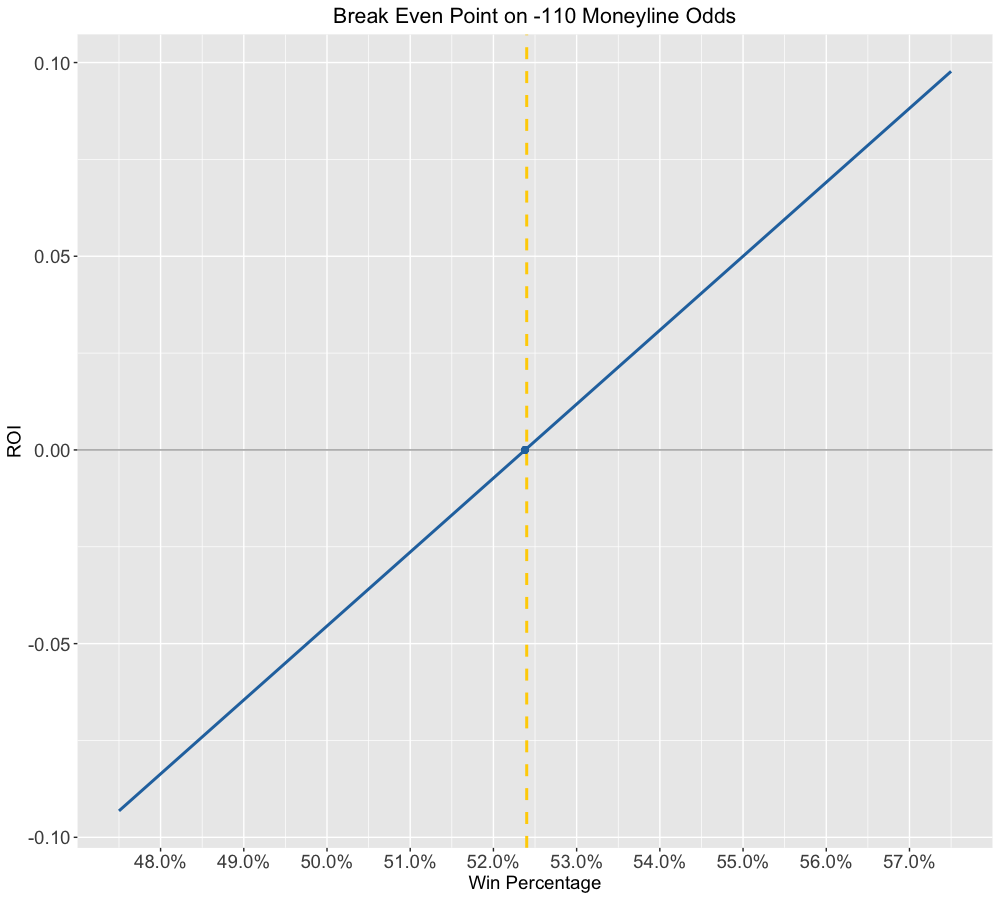
\includegraphics[width=4.5in]{break-even.png}
  \end{minipage}%
  \begin{minipage}[c]{0.10\linewidth}
    \vspace{0pt}
    \centering
    \footnotesize
        \begin{tabular}{@{}rrr@{}}
        \toprule
        Win \% & EV & ROI  \\ \midrule
        48\% & \$             (9.20) & -8.36\% \\
        49\% & \$             (7.10) & -6.45\% \\
        50\% & \$             (5.00) & -4.55\% \\
        51\% & \$             (2.90) & -2.64\% \\
        52\% & \$             (0.80) & 0.73\% \\
        53\% & \$              1.30 & 1.18\% \\
        54\% & \$              3.40 & 3.09\% \\
        55\% & \$              5.50 & 5.00\% \\
         \bottomrule
        \end{tabular}
   \end{minipage}
   \caption{Break even point based on expect return on investment for a -110 moneyline odds bet}
   \label{fig:exp-val}
\end{figure}

\normalsize

The break-even point is defined as the point where your ROI at a certain win probability goes from an expected loss to an expected gain. This point is clearly shown in Figure \ref{fig:exp-val} right at the magic 52.4\% number. So as long as sportsbooks continue to take their 10\% cut and place coin-flip games at -110 odds, bettors will have to win 52.4\% to keep their bankroll from slowly draining. Another quick way to get to this break-even point is by plugging a -110 moneyline into our implied probability formula.\\

\noindent \underline{Implied Win Probability of a -110 moneyline:}
\begin{flalign*}
IP(ML) & = \frac{(-1 * ML)}{(-1 * ML) + 100}  &\\
IP(ML) & = \frac{(-1 * -110)}{(-1 * -110) + 100}  \\
IP(ML) & = \frac{110}{110 + 100}  \\
IP(ML) & = .5238
\end{flalign*}

In short, bettors who win more than 52.4\% of their bets will ``beat the market'' and thusly their portfolio increases over time. Those that fall below the threshold will trend toward the negative.

Quick note: the table in Figure \ref{fig:exp-val} shows an ROI of -4.55\% at a win probability of 50\%. This essentially defines the casino's vig when placing their cut at 10\%. Given an even odds matchup (50\%), a sportsbook, on average, will take a 4.55\% vig from the betting pool.

\section{Fixed Bet Implementation}

This magic 52.4\% metric for sports bettors is most applicable when wagering on spreads, over/unders, or even-money games. These make up the most common wagers placed at sportsbooks and therefore that magic number is critical for high volume gamblers. But for the purposes of this study, however, we are analyzing moneylines which have varying profits based on the extent each team is a favorite or underdog. So in order to best gauge the success of our model, we can first test and implement two distinct fixed bet wagering strategies.

The first is the most intuitive, but potentially not the most lucrative. Option one is to look at the percent chances our model predicts a given team has to win the game and always pick the favorite. Basically, if the model predicts a win probability greater than 50\%, then we bet on that team. (This is the technique that was used when performing model performance analysis back in Chapter 5). This is also, more or less, how a casual bettor approaches making a wager. Upon looking at a matchup, one tries to predict which team is more likely to win (or that they want to root for) and then proceed to bet on them, regardless of where the betting odds lie.

The second option looks not just at who is more likely to win, but directly compares the chances that team will win versus the chances the sportsbook gives that team. A casual bettor might only have an inkling one way or the other, but because our model outputs a numerical win probability, we are able to put an exact amount on the discrepancy between the book and the model. For example, if Las Vegas thinks a team in a 90\% favorite (-900 odds), but our model predicts the team actually only has a 75\% chance of winning, we would actually bet on the opposing team. Although betting on a team that might not win is a risky proposition, the payout is higher for an underdog and that increased profit potential justifies the strategy. If the model was accurate enough, over time, exploiting this discrepancy between betting odds and model odds could be the edge a bettor needs to drive up their portfolio value. 

Figure \ref{fig:fixed-bet} depicts the logic flow for these two betting options when applied to a matchup between a hypothetical team (a favorite at a -235 moneyline) and its opponent (an underdog at a +185 moneyline).

\begin{figure}%
    \centering
    {{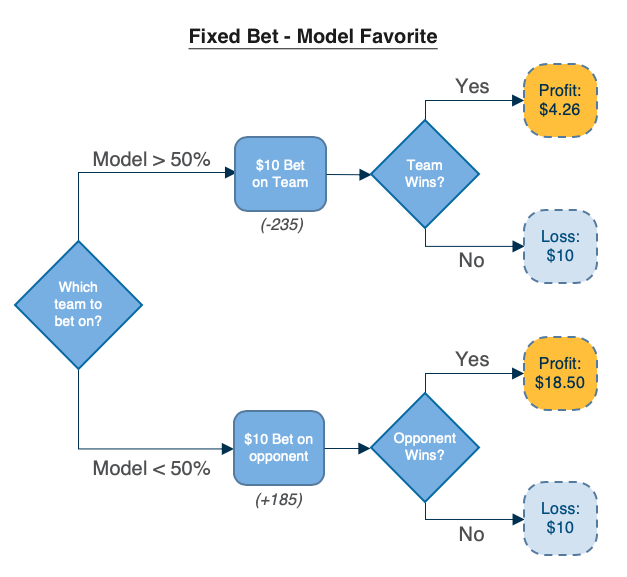
\includegraphics[width=7.75cm]{fixed-bets-fav.png} }}%
    \qquad
    {{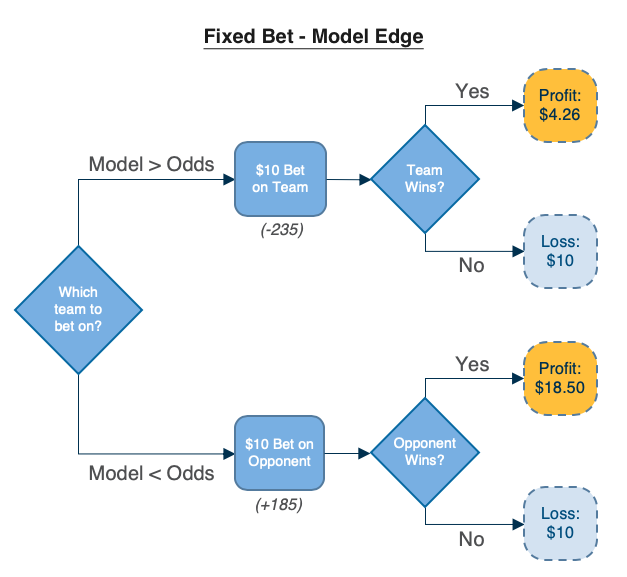
\includegraphics[width=7.75cm]{fixed-bets-edge.png} }}%
    \caption{Our two fixed bet wagering implementations}%
    \label{fig:fixed-bet}%
\end{figure}

\section{Bet Results on the Validation Set}
In order to test our model's performance in a real world betting application, we applied our wagering methodologies to the 2019-20 NBA season. Since our data was optimized based on a dataset from 2007-08 to 2018-19, the best way to get a true gauge of how it would perform in the wild  was to throw the model at an entirely new dataset. For these fixed rate betting methodologies, we place a \$10 wager on every single matchup based on the betting logic as defined in Figure \ref{fig:fixed-bet}. There are 1,230 games available to bet on in our dataset so the most once could lose in this testing experiment is \$12,300. Figure \ref{fig:bet-perf-fixed} indicates the results of the different betting methodologies. 

\begin{figure}[h]
\centering
  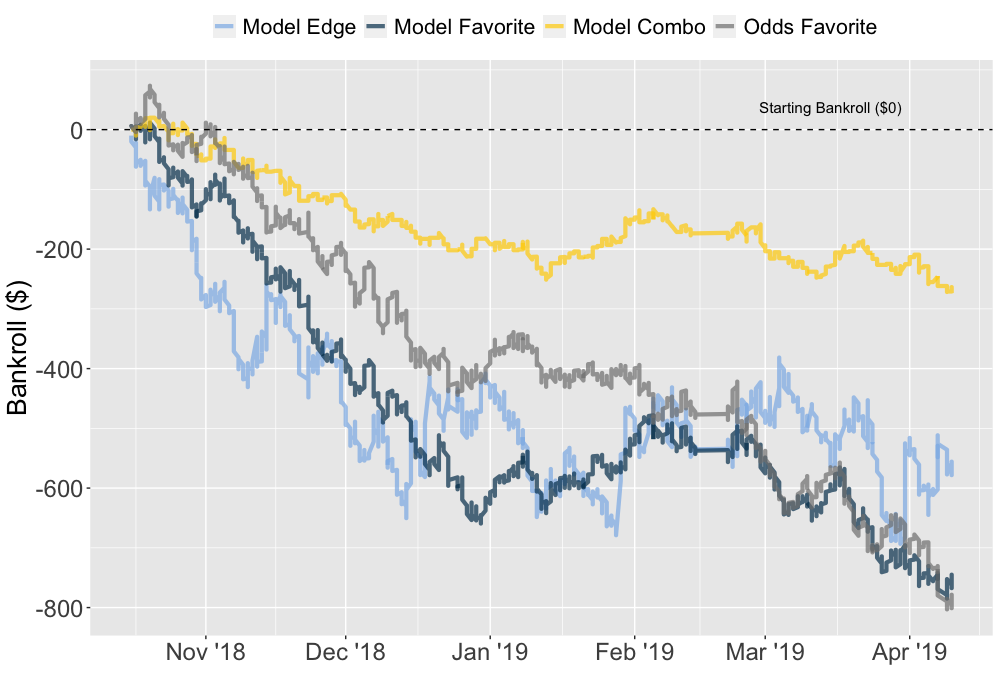
\includegraphics[width=450px]{bet-performance-fixed.png}
  \caption{Bankroll over time for betting results on odds from the 2019-20 NBA season}
  \label{fig:bet-perf-fixed}
\end{figure}

Also, just for interest, we decided to create somewhat of an ensembled betting strategy that was a combination of the two methods. Even if a bettor believes that a team is being undervalued in a matchup, it does not necessarily mean he should bet on that team. Let's say the sportsbook gives the team a 5\% chance of winning (+1900 moneyline) and our model predicts a 25\% chance. Even though this discrepancy is large, and there appears to be a considerable edge to exploit, the model still predicts that team will lose three times out of four. So even with the large profit for picking such an underdog, a risk-averse bettor might still avoid betting on that team. As a third betting method we used a ``model combo'' strategy where it will only place a wager if (1) the model predicts the existence of an edge and (2) the model predicts a greater than 50\% chance. If there is no edge or the predicted win probability is below 50\% it will choose to place no wager on the matchup.

In addition to comparing the three betting methodologies against each other (``model edge'', ``model favorite'', and ``model combo''), it seemed worthwhile to see how this model faired against the most conservative possible betting approach that was devoid of any recommendations from a betting model. That is, betting on the favorite team in each matchup as defined by the team with the sportsbook odds' win probability greater than 50\%. We see that this betting strategy actually loses a considerable amount of money over the course of the season. One would think that betting on the Vegas favorite (and winning about two-thirds of the time) would lead to a net profit. However, because of the structure of a moneyline, the profit from betting on a favorite can never be larger than the original risk. So each loss brings the bankroll down by an amount equal to the amount wagered, while each win can only bring the bankroll up by a smaller margin than the wager. Thus, winning over two-thirds of the games was not enough to overcome these conservative returns. We see a similar effect occurring with the ``model combo'' method as the gains are minimal while the losses are consistent.

Table \ref{tab:bet-results} summarizes the results from all four betting methodologies discussed as applied to the 2019-20 NBA dataset.

\begin{table}[]
\centering
\caption{Summary Results between Betting Methodologies}
\label{tab:bet-results}
\begin{tabular}{@{}lccccc@{}}
\toprule
 & Win & Loss & No Bet & Win Pct & Final Bankroll \\ \midrule
Model Favorite & 812 & 418 & - & 66.0\% & \$ -754.99 \\
Model Edge & 601 & 629 & - & 48.9\% & \$ -575.73 \\
Model Combo & 221 & 133 & 876 & 62.4\%  & \$ -273.63 \\ 
Odds Favorite & 818 & 394 & 18 & 67.5\% & \$ -788.54 \\ \bottomrule
\end{tabular}
\end{table}

%      Chapter 8    %%%%%%%%%%%%%%%%%%%%%%%%%%%%%%%%%%%%%%%%%%%%%%%%%%%%%%%%%%%%
\chapter{The Kelly Criterion}

In an effort to push our model evaluation even further and determine its most effective application, we researched more complex betting methodologies than simply wagering a fixed amount on each game. Intuitively we know that not all matchups are created equal. If a bettor was extremely certain about the outcome of a game, he should not wager the same amount as he would on a matchup he was less confident in. Again, the goal of a robust betting model would be to identify opportunities to gain an edge over the betting line. If our model predicted a team had a 80\% chance to win a game, but the sportsbook predicted the team had only a 40\% chance, this would be a prime opportunity to capitalize on this probability discrepancy and bet big. Research into a type of wagering methodology that could account for optimizations based on betting confidence led straight to the famous scientific gambling strategy known as the \emph{Kelly criterion.}

The formula was discovered in the mid-1950's by scientist J. L. Kelly, Jr. who was actually conducting research in analyzing long-distance telephone signal noise. However, its application was then adopted by economists and horse gamblers as a way to maximize portfolio profit and diversification. Over time, and more recently, Kelly strategy has become a part of mainstream investment theory and used by successful investors including notable billionaires such as Berkshire Hathaway's Warren Buffett and Charlie Monger and bond trader, Bill Gross. In brief, the Kelly criterion is the mathematical formula for investors and gamblers that calculates what percentage of their budget they should allocate to each investment or bet. \cite{kelly} By using the Kelly criterion a bettor would know exactly how much more to wager on bets that come with a high degree of confidence and the extent to avoid ones with low confidence, thus resulting in limiting losses and maximizing gains.

Although, partially out of the scope of this study, our betting model provides an ideal use case for the application of the Kelly criterion. We have a set of implied probabilities defined by the betting odds, another set of prediction probabilities, and the goal of maximizing profits based on the discrepancy between the two. As a result, for the final evaluation of our model and betting methodologies, it seemed worthwhile to take a brief tangent into applying the Kelly criterion on our 2019-20 NBA dataset to see if we could improve upon the results from Chapter 7's fixed bet strategies. But before utilizing the Kelly methods, we first need to understand its derivation.

\section{Deriving the Kelly Criterion}

In order to calculate the Kelly criterion, the following pieces of information are required for the formula:

\begin{itemize}
  \setlength\itemsep{-0.75em}
\item \emph{p}: true probability of an event
\item \emph{q}: probability the event does not occur \emph{(q = 1 - p)}
\item \emph{b}: given odds of the event occurring (in the format of \emph{``b to 1''})
\end{itemize}

The Kelly criterion (\emph{k}) is defined using those three variables in the following formula:

\begin{equation}\label{eq:kellyc}
k = \frac{pb - q}{b}
\end{equation}

If \emph{k} is positive, you make the size of your wager equal to \emph{k} percentage of your entire bankroll. If \emph{k} is negative, you do not make the wager. So where does this formula come from? The answer, which makes sense in context, is derived from finance and the equations for a compounding bankroll model and compound growth rate. \cite{youtube}

\subsection{The Compounding Bankroll Model}
The economics behind the compounding bankroll model can be applied to any type of bankroll growth whether it's the stock market or gambling. All that is needed is some form of binary outcomes that can be defined as a ``win'' versus a ``loss''. The equation essentially takes your initial bank amount and increases the bankroll for each win and decreases it for every loss. The degree to which it goes up or down is a function of how much you risk and how likely a win is versus a loss. See Equation \ref{eq:cbm}.

\begin{center}
\underline{Compounding Bankroll Model}
\begin{equation}\label{eq:cbm}
A_n = A_0 (1 + bk)^W (1-k)^L
\end{equation}
\end{center}

\begin{itemize}
  \setlength\itemsep{-0.75em}
\item \emph{$A_n$} = amount of money (in dollars) after n bets
\item \emph{$A_0$} = starting amount of money (initial bankroll)
\item \emph{n} = total number of bets, with \emph{n = W + L}
\item \emph{$W$} = number of winning bets
\item \emph{$L$} = number of losing bets
\item \emph{$k$} = fraction of  bankroll to be wagered
\item \emph{$b$} = current odds against (stated as \emph{``b to 1''})
\end{itemize}

The following is a brief example of how to utilize Equation \ref{eq:cbm}. Say you have \$100 in your account (i.e. \emph{$A_0$} = 100). The given odds of winning are 2:1 (\emph{b} = 2) and you intend to wager 10\% of your bankroll on each bet (k = 10\%). Find the rate of change of your bankroll.
\begin{flalign*}
A_n &= A_0 (1 + bk)^W (1-k)^L &\\
A_n &= 100(1 + 2(0.1))^W (1-0.1)^L\\
A_n &= 100(1.2)^W(0.9)^L
\end{flalign*}

Therefore, if you bet 10\% of your bankroll at the given 2:1 odds, with each ``win'' the bankroll will increase by 20\% and with each `loss'' it will decrease by 10\%. If you made four wagers and had two wins and two losses, it would result in a final balance of about \$117 which is a 17\% rate of return.
\begin{flalign*}
A_n &= 100(1.2)^2(0.9)^2 &\\
A_n &= 100(1.44)(0.81) \\
A_n &= 116.64
\end{flalign*}

\subsection{Compounding Growth Rate}
In order to maximize a compounding bankroll, we need to optimize the rate in which that bankroll increases. The way to calculate this rate of return is with an equation for compounding growth rate per bet. Equation \ref{eq:cgr} is the standard formula for compound growth rate applied to any type investment or financial return. Usually \emph{n} is notated as \emph{t} to reflect the amount of time the return in accumulating over, but for the purposes of this application, we use \emph{n} to indicate how many wagers the growth accumulated over.

\begin{center}
\underline{Compounding Growth Rate}
\begin{equation}\label{eq:cgr}
G = \left( \frac{A_n}{A_0}\right )^\frac{1}{n} - 1
\end{equation}
\end{center}

Again, a brief example on the application of this formula. Say a bettor made four wagers and his bankroll increased from \$100 to \$150 over the course of those bets. Find the growth rate over this time period.
\begin{flalign*}
A_0 &= 100, A_4 = 150, n = 4 & \\
G &= \left( \frac{150}{100}\right )^\frac{1}{4} - 1 \\
G &= (1.5)^\frac{1}{4} - 1 \\
G &= 1.1067 - 1 \\
G &= 10.67\%
\end{flalign*}

So this bettor had a 50\% return on investment ($\frac{150-100}{100}$) with a compound growth rate of 10.65\% per bet.

\subsection{Maximizing growth rate}
Finally, to get to our goal of deriving the Kelly criterion we need to put these two concepts together and optimize for the per bet rate of return (\emph{G}). This would tell us, based on all the given information about the likelihood of winning or losing a bet, the optimal fraction of the bank to wager. To get this value we plug the compound growth rate equation into the compound bankroll model. Then, like we do with all maximizations, we take the derivative and set it equal to 0. \\

\centerline{\underline{Optimizing for Growth Rate}}
\noindent Goal: seek a value for \emph{k} such that it will maximize the per bet rate of return (\emph{G}) \\
$\text{Given: G =} \left( \frac{A_n}{A_0}\right )^\frac{1}{n} - 1 \text{  and  } A_n = A_0 (1 + bk)^W (1-k)^L$
\begin{equation*} \label{eq:kc-deriv}
\begin{split}
A_n &= A_0 (1 + bk)^W (1-k)^L \\
\frac{A_n}{A_0} &= (1 + bk)^W (1-k)^L \\
\left(\frac{A_n}{A_0}\right)^\frac{1}{n} &= \left[(1 + bk)^W (1-k)^L\right]^\frac{1}{n} \\
&= (1+bk)^\frac{W}{n}(1-k)^\frac{L}{n}
\end{split}
\end{equation*}

\noindent \text{Let p = $\frac{W}{n}$ be the true probability of winning} \\
\noindent \text{Let q = $\frac{L}{n}$ be the true probability of losing}
\begin{equation*}
\begin{split}
\left(\frac{A_n}{A_0}\right)^\frac{1}{n} = (1+bk)^p(1-k)^q 
\end{split}
\end{equation*}

Basic algebra allows us to declare that $(1+bk)^p(1-k)^q = e^{ln[(1+bk)^p(1-k)^q]}$. Therefore, $\left(\frac{A_n}{A_0}\right)^\frac{1}{n}$ is maximized when $ln[(1+bk)^p(1-k)^q]$ is maximized as well. 
\begin{equation*} \label{eq:kc-deriv2}
\begin{split}
\text{Let } f(k) &= ln[(1+bk)^p(1-k)^q] \\
&= ln(1+bk)^p + ln(1-k)^q \\
&= p \cdot ln(1-bk) + q \cdot ln(1-k) \\
f'(k) &= p \cdot \frac{1}{1+bk} \cdot b + q \cdot  \frac{1}{1-k} \cdot  -1 \\
&= \frac{pb}{1+bk} + \frac{-q}{1-k} 
\end{split}
\end{equation*}

Then, to find our critical point...

\begin{equation*} \label{eq:kc-deriv3}
\begin{split}
f'(k) &= \frac{pb}{1+bk} - \frac{q}{1-k} = 0 \\
\frac{pb}{1+bk} &= \frac{q}{1-k} \\
pb(1-k) &= q(1+bk) \\
pb - pbk &= q + qbk \\ 
pb - q &= pbk + qbk \\ 
pb - q &= k(pb + qb) \\
k &= \frac{pb-q}{(pb+qb)} \\ 
k &= \frac{pb-q}{b(p+q)} \hspace{1.5cm} \text{  ... since p+q = 1} \\
k &= \frac{pb-q}{b}
\end{split}
\end{equation*}

Finally, to ensure this critical point is indeed a maximum, and not a minimum, we take the second derivate and set equal to 0...
\begin{equation*} \label{eq:kc-deriv3}
\begin{split}
f'(k) &=\frac{pb}{1+bk} = \frac{q}{1-k}  \\
f''(k) &= \frac{-pb^2}{(1+bk)^2} - \frac{q}{(1-k)^2} = 0\\
\end{split}
\end{equation*}

We know the denominator on both terms will always be positive. Also we know p and q are always positive. Therefore we have a negative term minus a positive term which will always result in a negative number. So we can conclude $f''(k) < 0$ and therefore $f'(k)$ is indeed a maximum of our function.

\subsection{Example application of the Kelly Criterion}
So the formula is now derived for the optimal amount to wager such that it maximizes the rate of return of our portfolio: $k = \frac{pb-q}{b}$. Applying this equation to an example wagering scenario is straightforward as we now have all the variables required to test this formula.

Let's say you wanted to bet on a team with -110 moneyline odds (recall that comes out to the 52.4\% implied probability discussed earlier). Now say our model believes the true win percentage for that team is actually 55\%. Find the optimal wager amount (the Kelly criterion) as a fraction of your total bankroll.

First we need to convert the moneyline into odds (\emph{b}) so that it is formatted as \emph{``b to 1''}. Converting moneylines to odds is simple:

\begin{center}
\text{\underline{Moneyline to Odds Conversion - General Equation}}
\begin{equation} \label{ml_to_odds}
\text{Odds = }
\begin{cases}
\displaystyle
 \frac{ML}
 {100},  & \text{if ML} \geq 0 \\ \\ 
\displaystyle
 \frac{100}
 {-1 * ML}, &  \text{if ML} <  0\\ 
\end{cases}
\end{equation}
\end{center}

So for our example problem we have:
\begin{itemize}
  \setlength\itemsep{-0.75em}
\item \emph{p}: true probability of an event = 55\%
\item \emph{q}: probability the event does not occur  = 45\%
\item \emph{b}: given odds of the event occurring = $\frac{100}{110}$ = .909
\end{itemize}

Input these variables into the Kelly criterion formula and we get...
\begin{equation*} 
\begin{split}
k &= \frac{pb-q}{b} \\
k &= \frac{0.55*0.909 - 0.45}{0.909} \\
k &= \frac{0.4995}{0.909} \\
k &= 0.05495
\end{split}
\end{equation*}

Therefore, the optimal wager would be to place about 5.55\% of your total bankroll on this bet to ensure the maximum long term growth rate. We can even see what the expected compound bankroll growth would be if, for example, we wagered 20 times, winning 11 and losing 9.
 \begin{flalign*}
A_n &= 100(1 + bk)^W(1-K)^L & \\
& = 100(1 + (0.909)(0.0555))^{11}(1-0.0555)^9 \\
& = 100(1.0505))^{11}(.9445)^9 \\
& = 102.85 
\end{flalign*}

The portfolio went from a starting bankroll of \$100 to \$102.85 over the course of the 20 bets. Even though this growth rate seems small at 2.85\%, we achieved this growth winning only one more game than we lost. A consistent growth rate of almost 3\% from a win percentage of just 55\% percent could lead to hefty returns over the course of a large sample size of bets.

One final note on the definition of the Kelly criteria. We could rewrite the formula as such:
\begin{equation*} 
\begin{split}
k &= \frac{pb-q}{b} \\
k &= \frac{p(b) - q(1)}{b}
\end{split}
\end{equation*}

The numerator \emph{p(b) - q(1)} can be translated to simply the ``expected value on a \$1 bet.'' This expression breaks down as follows: the probability of winning, multiplied by the betting odds, minus the probability of losing, multiplied by the betting risk. We've been referring to the concept of trying to find \emph{the betting edge} throughout this research. So formally, within the gambling sphere, this edge is defined as the expected value on a \$1 bet. Essentially, over time, how much do you expect to profit (or lose if it equates to a negative value) from this wager. Thusly, one could also refer to the formula for the Kelly criterion as:
\begin{equation*} 
k = \frac{\text{expected value on a \$1 bet}}{\text{odds}} = \frac{\text{edge}}{\text{odds}}
\end{equation*}


\section{Applying the Kelly Strategy to our Data}

The implementation of the Kelly criterion to our dataset was similar to the ``model edge'' fixed betting strategy conducted in Chapter 7 as they both involved identifying the discrepancy between the model's predicted win probability and the implied probability from the betting odds. In fact, the logic flow to utilize the Kelly criterion is actually the same as the ``Fixed Bet - Model Edge'' defined in Figure \ref{fig:fixed-bet}, but instead of placing a \$10 stake on either the team or the opponent, that wager would be variable. 

First, we had to define an initial bankroll amount, which we set at \$1,000. Then, for every matchup, we compared the model probability to the team's win probability as defined by its moneyline. If the odds were better than the probability we would wager on that team, it it was worse then we would wager on the opponent. Next was the calculation of how much to wager based on the Kelly criteria. If the model recommended betting on the team, we'd plug the model probability in for \emph{p}, betting odds in for \emph{b}, and the moneyline converted probabilities for \emph{p} and \emph{q}. This gave us the value, \emph{k}, which defined the fraction of the present bankroll to wager. If the model probability was worse than the betting probability for the team, then we'd just apply the same technique, but instead do so to the opponent's variables. Again using the same 1,230 games from the 2019-20 NBA season, we can see how the initial \$1,000 bankroll fluctuated over the series of bets.

One of the common critiques to the Kelly wagering strategy is that it is oftentimes too aggressive. Although, mathematically the derivation does suggest that the technique, over a large enough sample size, does trend toward an optimal expected value. The issue, however, is that the model is so heavily reliant on the values inputted as the ``true probability'' (\emph{p}). So the strategy can only be as effective as the model is accurate. Additionally, Kelly-based strategies are extremely high variance. If the identified edge is extremely large, the Kelly criterion will recommend almost the entire bankroll. This is a great strategy to rapidly compound your portfolio if the prediction comes to be out be true. But an unforeseen circumstance leading to an instance of bad fortune can cripple the account with one large failed wager. And because the Kelly wagering method is a function of your total bankroll, once that account is extremely low, it takes exponentially longer to drive it back upwards.

As a result, remedies have been developed to counteract the high variance troubles associated with such an aggressive betting strategy. One of the recommendations to smooth out the wild oscillations common to Kelly-based wagering is to use the concept of ``fractional Kellys''. \cite{thorp} For example, if the formula outputted the optimal wager for a certain matchup was 40\% of the present bankroll, a bettor might be weary about such an aggressive bet. So instead, a fractional Kelly would recommend betting half of the formula's result or just a quarter of it (20\% of the bankroll or 10\%, respectively). Wagering with a fractional Kelly still allows for the bettor to increase or decrease their wager amount systematically based on their confidence in the existence of a betting edge, but doing so with a more tempered approach. Figure \ref{fig:bet-perf-kc} illustrates the results from using four variations of the Kelly criteria on our validation data set from the 2019-20 NBA season. Ranging from most conservative to most aggressive, we utilized a ``Quarter Kelly'', ``Third Kelly'', ``Half Kelly'', and ``Full Kelly''.

\begin{figure}[h]
\centering
  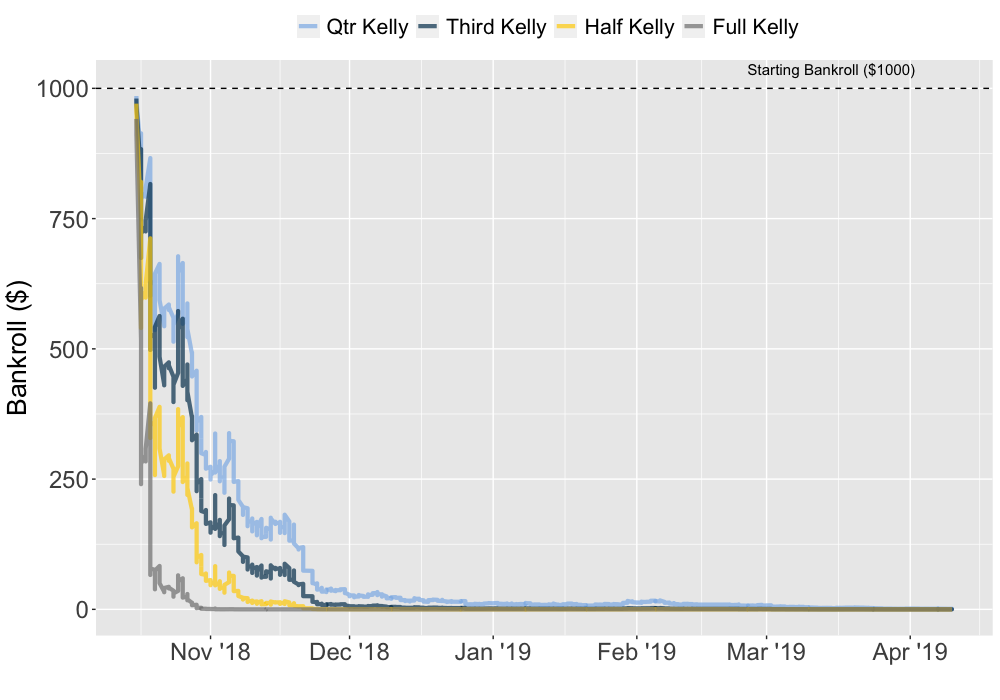
\includegraphics[width=450px]{bet-performance-kc.png}
  \caption{Bankroll over time using various Kelly criteria for the 2019-20 NBA season}
  \label{fig:bet-perf-kc}
\end{figure}

Unfortunately, all four betting methodologies ended up trending toward a final bankroll of \$0. It of course could never reach \$0 as the wager amount is a fractional value relative to the total bankroll. But in a real life scenario, casinos have a minimum bet amount that one can wager on a matchup (usually around \$5), so the Kelly criteria could be utilized in its empirical form up until the wager dropped below that minimum amount, in which case you would probably have to go ``all in'' as they say in poker. As expected, we see that as each fractional Kelly decreases in size (i.e. becomes more conservative), the longer it takes for the bankroll to bottom out. As we would also expect, the win-loss record of the Kelly implementation was the exact same as the ``Model Edge'' method summarized in Table \ref{tab:bet-results}. Again, the difference between the two methodologies was in the amount wagered and whether it was the fixed rate or the variable (and theoretically optimal) amount defined by the Kelly criterion. 

Although utilizing the Kelly criteria betting strategy did not yield vastly improved results from the fixed rate methods in Chapter 7, the experiment was worthwhile. In theory, this technique does have the potential to compound positive results rapidly if the model was particularly performant. But in practice, the Kelly method is only as powerful as the quality of its parameters. What we learned is that these high-variance strategies should be reserved for opportunities with a more robustly built and reliable model to use as the ``true probability'' input into the Kelly criteria formula.

%      Chapter 10     %%%%%%%%%%%%%%%%%%%%%%%%%%%%%%%%%%%%%%%%%%%%%%%%%%%%%%%%%%%%
\chapter{Conclusions}


%      Chapter 11     %%%%%%%%%%%%%%%%%%%%%%%%%%%%%%%%%%%%%%%%%%%%%%%%%%%%%%%%%%%%
\chapter{Appendix}

Lorem ipsum dolor sit amet, consectetur adipiscing elit.

\begin{table}[]
\centering
\caption{League Average Stats per Game by Season}
\label{tab:season-avgs}
\begin{tabular}{@{}llll@{}}
\toprule
Season & Points & Field-Goal Att & Three-Point Att \\ \midrule
2007-08 & 99.9 & 81.5 & 18.1 \\
2008-09 & 100.0 & 80.9 & 18.1 \\
2009-10 & 100.4 & 81.7 & 18.1 \\
2010-11 & 99.6 & 81.2 & 18.0 \\
2011-12 & 96.3 & 81.4 & 18.4 \\
2012-13 & 98.1 & 82.0 & 19.9 \\
2013-14 & 101.0 & 83.0 & 21.5 \\
2014-15 & 100.0 & 83.6 & 22.4 \\
2015-16 & 102.7 & 84.6 & 24.1 \\
2016-17 & 105.6 & 85.4 & 27.0 \\
2017-18 & 106.3 & 86.1 & 29.0 \\
2018-19 & 111.2 & 89.2 & 32.0 \\
2019-20 & 111.4 & 88.8 & 33.9 \\ \bottomrule
\end{tabular}
\end{table}



\bibliography {tes} 
\bibliographystyle {uclathes}
%\bibliography {bib/network,bib/naming}    % bibliography references
%\bibliographystyle {thesis}

\end {document}
